\documentclass[12pt,a4paper]{book}
\usepackage[utf8]{inputenc}
\usepackage[spanish,es-noshorthands]{babel}
\usepackage{amsmath}
\usepackage{amsfonts}
\usepackage{amssymb}
\usepackage{latexsym}
\usepackage{makeidx}
\usepackage{graphicx}
\usepackage{graphics}
\usepackage{lmodern}
\usepackage{hyperref}
\usepackage{subcaption}
\usepackage{pgfplots}
\usepackage{dsfont}
\usepackage{amsthm}
\usepackage{multicol}
\usepackage{xcolor}
\usepackage{booktabs}
\usepackage{float}
\usepackage{subcaption}
\pgfplotsset{width=10cm,compat=1.9}
\usepgfplotslibrary{external}
\usepackage{fancybox}


\setlength{\parindent}{12px}
\usepackage[left=2cm,right=2cm,top=4cm,bottom=2cm]{geometry}

\author{Daniel Vázquez Lago}
\title{Apuntes Métodos Matemáticos VI}

\newcommand{\parentesis}[1]{\left( #1  \right)}
\newcommand{\parciales}[2]{\frac{\partial #1}{\partial #2}}
\newcommand{\pparciales}[2]{\parentesis{\parciales{#1}{#2}}}
\newcommand{\ccorchetes}[1]{\left[ #1  \right]}
\newcommand{\D}{\mathrm{d}}
\newcommand{\derivadas}[2]{\frac{\D #1}{\D #2}}
\newcommand{\sech}{\mathrm{sech} \ }
\newcommand{\csch}{\mathrm{csch} \ }
\newcommand{\cotanh}{\mathrm{cotanh}}
\newcommand{\cotan}{\ \mathrm{cotan}}
\newcommand{\Res}{\mathrm{Res}}
\newcommand{\Real}{\mathrm{Re}}
\newcommand{\Arg}{\mathrm{arg}}
\newcommand{\inti}{\int_{-\infty}^{\infty}}
\newcommand{\into}{\int_{0}^{\infty}}
\newcommand{\hatf}{\widehat{f}}
\newcommand{\tf}{\tilde{f}}

\newcommand{\tquad}{\quad  \quad \quad}

\newtheorem{theorem}{Teorema}[section]
\newtheorem{corollary}{Corolario}[theorem]
\newtheorem{lemma}{Lema}[section]
\newtheorem{ejemplo}{Ejemplo}[section]

%\theoremstyle{definition}
\newtheorem{definicion}{Definición}[section]

\begin{document}

\maketitle

\newpage

\tableofcontents

\newpage


\newpage


\chapter{Plano complejo}

\section{Introducción}

La solución de ecuaciones algebraicas cuadráticas y cúbicas (o de orden mayor) nos llevan muchas veces a raíces negativas. La ecuación mas famosa es:

$$ x^2 + 1 = 0 \Longrightarrow x= \pm \sqrt{-1} $$

Esto llevo a los matemáticos a crear una nueva forma de resolver esta clase de problemas fuera de la variable real (ya que en la recta real este problema no tiene solución). Aparecen así los números complejos, que mas allá de ser una simple solución a problemas algebraicos aparecen en la la mayoría de los campos de la física tales como la mecánica cuántica, y nos sirven incluso para resolver integrales, ecuaciones diferenciales, integrables... 

\section{El cuerpo de los números complejos}

La mayoría ya hemos sido introducidos brevemente en los números complejos, por lo que no resultará ningún problema la mayoría de conceptos que vamos a mencionar aquí, que simplemente haremos para que el lector tenga una referencia, o que si surje alguna duda se pueda consultar rápidamente. \\

Un número complejo $z$ está definido por dos partes, por una real y por otra imaginaria, de manera muy similar al plano cartesiano $\mathbb{R}^2$. Entonces $z$ se puede definir como

\begin{equation}
z  =x + iy = (x,y)
\end{equation}

donde $x$ es la unidad real e  $i y$ es la unidad imaginaria, tal que $i$ viene dada por:

\begin{equation}
i = \sqrt{-1}
\end{equation}

y viene representado en el plano cartesiano en el eje $y$. En general podemos entender un número complejo como un plano cartesiano con propiedades únicas. La manera de sumar números complejos es análoga al plano cartesiano (así como la resta, la multiplicación por escalares reales...), pero el producto de números complejos es completamente nuevo, y viene dado por:

\begin{equation}
z_1 \cdot z_2 = (x_1,y_1) \cdot (x_2,y_2) = (x_1 x_2 - y_1 y_2, x_1 y_2 + y_1 x_2)
\end{equation}

de hecho la manera de representarlos como $x+iy$ es casi una manera de describir esta propiedad sin mencionarla, ya que si $z_1 = x_1+ i y_1$ y $z_2 = x_2 + i y_2$ y los multiplicamos como haríamos normalmente obtenemos el mismo resultado. \\

En el plano complejo son muy importantes los \textbf{complejos conjugados}. Sea $z$ un número complejo $x+iy$, llamamos al conjugado de $z$ como $\bar{z}$ al número

$$ x -iy $$

\section{Forma polar}

La forma polar de un número complejo es sumamente interesante, ya que permite facilitar cálculos a la hora de jugar con los exponentes, multiplicaciones entre números complejos... además de que te permite calcular expresiones como $\sin (2 \theta)$ en un minuto. \\

Entonces: 

\begin{equation}
x = r \cos \theta, \quad y = \sin \theta, \quad 0 \leq r < \infty, \quad 0 \leq \theta < 2 \pi
\end{equation}

Se denomina \textbf{módulo} o valor absoluto de $z$ al término $r$, denotado como $|z|$, y fase o \textbf{argumento} de $z$ a $\theta$, llamado muchas veces $\Arg{z}$. Definimos:

\begin{equation}
r = \sqrt{x^2 + y^2}; \quad \theta = \arctan (y/x)
\end{equation}

Entonces la fórmula polar de un número complejo:

\begin{equation}
z = r(\cos \theta + i \sin \theta)
\end{equation}

\section{Fórmula de De Moivre}

Si tomamos dos números complejos expresados en su forma polar y hacemos el producto está claro que:

\begin{equation}
z_1 z_2  = r_1 r_2 [\cos (\theta_1 + \theta_2 + i \sin (\theta_1 + \theta_2))]
\end{equation}

y para el producto de $n$ números complejos podemos hallar que:

\begin{equation}
z_1 \cdots z_n = r_1 \cdots r_n [\cos (\theta_1 + \cdots + \theta_n ) + i \sin(\theta_1 + \cdots + \theta_n )]
\end{equation}

y por lo tanto es trivial la \textbf{fórmula de De Moivre:}

\begin{equation}
z^n = r^n [\cos(n \theta)+i\sin(n \theta)]
\end{equation}

\section{Raíces de números complejos}

Un número $w \in \mathbb{C}$ se dice que es una raíz enésima de $z$, si $w^n=z$ tal que $n \in \mathbb{N}$. En este caso:

\begin{equation}
w = z^{1/n}
\end{equation}


Entonces usando la fórmula de De Moivre obtenemos que si $z \neq 0$ existen $n$ raíces $n$-ésimas tenemos que:

\begin{equation}
z^{1/n} = r^{1/n} \ccorchetes{\cos \parentesis{\frac{\theta+2k \pi}{n}} + i \sin \parentesis{\frac{\theta + 2k \pi}{n}}}, \quad \quad k=0,1,\ldots,n-1
\end{equation}

Es muy sencillo de ver, ya que si nos fijamos si elevamos a $n$ dicha solución obtenemos que:

$$
z = r^{n/n} \ccorchetes{ \cos \parentesis{\frac{n \ \theta}{n}+ \frac{2 \pi k n}{n}} + i \sin \parentesis{\frac{n \ \theta}{n}+ \frac{2 \pi k n}{n}}, \quad \quad k=0,1,\ldots,n-1}$$

sabiendo que el $2k \pi$ hace que demos k vueltas al cero, pero como $\theta + 2k \pi = \theta$, podemos decir que

$$ z = r \ccorchetes{\cos(\theta) + \sin (\theta)} $$ 

es decir, lo que estábamos buscando. Una curiosidad es que las n-enésimas raíces de $1$ representan, geométricamente un polígono regular de $n$ lados inscritos en una circunferencia de radio unidad y centro el origen. 


\section{Forma exponencial de los números complejos}

Sabemos que la función exponencial $e^x$ se puede desarrollar en serie de taylor: 

\begin{equation}
e^x = \sum_{n=0}^{\infty} \dfrac{1}{n!} x^n 
\end{equation}

que podemos dividirlo en pares e impares:

\begin{equation}
e^x = \sum_{n=0}^{\infty} \dfrac{1}{(2n+1)!} x^{2n+1} + \sum_{n=0}^{\infty} \dfrac{1}{(2n)!} x^{2n} 
\end{equation}

Y si ahora escribimos $x=\theta i$ podemos ver que aparecerán números negativos cuando $n=2,3,6,7 \ldots$ y el número imaginario unidad $i$ para las exponenciales impares. Entonces:

\begin{equation}
e^{\theta i} = \sum_{n=0}^{\infty} \dfrac{(-1)^n}{(2n+1)!} x^{2n+1} + \sum_{n=0}^{\infty} \dfrac{(-1)^n}{(2n)!} x^{2n}  = \cos(\theta) + i \sin  (\theta)
\end{equation} 

esta fórmula se llama la \textbf{fórmula de Euler}, y permite representar de manera mucho mas sencilla las raíces $n$-ésimas de un número complejo:

\begin{equation}
z^{1/n} = r^{1/n} e^{i 2k \pi / n} \quad \quad k = 0,1,2,\ldots,n-1
\end{equation}

\chapter{Funciones de variable compleja}

\section{Variables y funciones}

Llamamos \textit{variable compleja} a cualquier elemento (simbolizado por $z$, $w \ldots$) que representa cualquier elemento de un conjunto de números complejos. \\

Si a cada valor que puede tomar la variable compleja $z$ le corresponde (asignamos al valor $z$) uno o más valores de una variable $w$, decimos que $w$ es una \textit{función} de $z$ y escribimos $w=f(z)$. La variable $z$ es denominada la \textit{variable independiente} y la variable $w$ la \textit{variable dependiente}.

\subsection{Funciones univocas y mutivocas}

Si a cada valor de $z$ corresponde sólo un valor de $w$, decimos que $w$ es una \textit{función unívoca} de $z$ o que $f(z)$ es unívoca. Si más de de un valor de $w$ corresponde a cada valor de $z$, decimos que $w$ es una \textit{función multívoca} de $z$. \\

Una función multievaluada puede considerarse como una colección de funciones unívocas, donde cada miembro es llamado \textit{rama} de la función.  \\


\shadowbox{\textbf{Ejemplo 2.1 y 2.2}}

\hrulefill
\begin{itemize}

\item \textbf{Ejemplo 2.1:} si $w = z^2$, entonces para cada valor de z existe un solo valor de $w$. Por lo tanto es una función univoca de z.

\item \textbf{Ejemplo 2.2:} si $w = z^{1/2}$, entonces para cada valor de $z$ existen dos valores de $w$. Por lo tanto es una función multívoca (bivaluada) de $z$. 

\end{itemize}
\hrulefill \\

\subsection{Trasformaciones}

Si $w = u +iv$ y $z = x+iy$ podemos considerar la función $w=f(z)$ como $u+iv = f(x+iy)$. Entonces como sabemos podemos escribir $x+iy $ como $(x,y)$ y entoncces la función $f$ es una función análoga a $\mathbb{R}^2 \rightarrow \mathbb{R}^2$. Es equivalente a:

\begin{equation}
u = u(x,y) \ \ v=v(x,y)
\end{equation}

Entonces a cada punto $(x,y)$ en el plano $z$, tal como $P$, le corresponde el punto $(u,v)$ en el plano $w$, digamos $P'$. Entonces decimos que en el punto $P$ se \textit{aplica o transforma} en el punto $P'$, llamado \textit{imagen} de $P$.

\subsection{Funciones elementales}


\begin{enumerate}

\item \textbf{Funciones polinomiales} son las definidas por

\begin{equation}
w = a_n z^n + \cdots + a_2 z^2 + a_1 z + a_0
\end{equation}

donde $a_n \neq 0, \ldots, a_2, a_1, a_0$ son constantes complejas.

\item \textbf{Funciones alegraicas racionales} son las definidas por 

\begin{equation}
w  = \dfrac{P(z)}{Q(z)}
\end{equation}

donde $P(z)$ y $Q(z)$ son polinomios.

\item \textbf{Funciones exponenciales} son las definidas por 

\begin{equation}
w = e^z = e^x (\cos y + i \sin y)
\end{equation}

Si $a$ es real y positivo definimos:

\begin{equation}
a^z = e^{z \ln a}
\end{equation}

\item \textbf{Funciones trigonométricas.} Definimos las funciones trigonométricas en términos de las funciones exponenciales:

\begin{equation}
\begin{array}{cclccclc}

\sin z & = & \dfrac{e^{iz}-e^{-iz}}{2i} & \ \ \ \ \ \ \ \ & \cos z & = & \dfrac{e^{iz} + e^{-iz}}{2} \\ \\

\sec z & = & \dfrac{1}{\cos z} = \dfrac{2}{e^{iz}+e^{-iz}} & \ & \csc z& = & \dfrac{1}{\sin z} = \dfrac{2i}{e^{iz}-e^{-iz}} \\ \\

\tan z & = & \dfrac{\sin z}{\cos z} = \dfrac{e^{iz}-e^{-iz} }{i (e^{iz}+e^{-iz})} & & \cot z & = & \dfrac{\cos z}{\sin z} = \dfrac{i(e^{iz}+e^{-iz})}{(e^{iz}-e^{-iz})} 

\end{array}
\end{equation}

La mayoría de las propiedades de las funciones trigonométricas reales son válidas para las funciones complejas, como

\begin{equation}
\sin^2 z + \cos^2 z = 1; \ \ \sin(-z) = - \sin(z); \ \ \cos (-z) = \cos (z) \ldots
\end{equation}

además de las funciones angulo doble, ángulo mitad... De hecho estas se pueden deducir directamente de las expresiones complejas.


\item  \textbf{Funciones hiperbólicas} son las definidas como


\begin{equation}
\begin{array}{cclccclc}

\sinh z & = & \dfrac{e^{z}-e^{-z}}{2} & \ \ \ \ \ \ \ \ & \cosh z & = & \dfrac{e^{z} + e^{-z}}{2} \\ \\

\sech z & = & \dfrac{1}{\cosh z} = \dfrac{2}{e^{z}+e^{-z}} & \ & \csch z& = & \dfrac{1}{\sinh z} = \dfrac{2i}{e^{z}-e^{-z}} \\ \\

\tanh z & = & \dfrac{\sinh z}{\cosh z} = \dfrac{e^{z}-e^{-z} }{ (e^{z}+e^{-z})} & & \coth z & = & \dfrac{\cosh z}{\sinh z} = \dfrac{(e^{z}+e^{-z})}{(e^{z}-e^{-z})} 

\end{array}
\end{equation}

Siendo las siguientes propiedades válidas

\begin{equation}
\cosh^2 z - \sinh^2 z = 1; \ \ \sinh (-z) = - \sinh (z); \ \ \cosh (-z) = \cosh (z) \ldots
\end{equation}


Lo mas destacable de estas funciones es que están relacionadas con las funciones trigonométricas, de la siguiente forma:

\begin{equation}
\sin iz = i \sinh z; \ \ \ \ \cos iz = \cosh z
\end{equation}

\item \textbf{Funciones logarítmicas.} Es la función inversa de la función exponencial, y es multivaluada ya que si $z = r e^{i \theta} = r e^{\theta + 2k \pi}$ tenemos que:

\begin{equation}
\ln z = \ln r + i (\theta + 2k \pi) \ \ \ k = 0, \pm 1, \pm2, \ldots
\end{equation}

En este caso la \textit{rama principal} de la función logaritmo se define para $k=0$, es decir:

\begin{equation}
\ln z = \ln r + i \theta
\end{equation}


\item \textbf{Funciones trigonométricas inversas.} Si $z = \sin w$, entonces $w = \sin^{-1}$ se llama \textit{seno inverso de z} o \textit{arcoseno de z}. Son todas ellas funciones multivaluadas, y se expresan en términos de logaritmos naturales:

\begin{equation}
\begin{array}{cclccclc}

\sin^{-1} z & = & \dfrac{1}{i} \ln (i z + \sqrt{1-z^2}) & \ \ \ \ \ \ \ \ & \cos^{-1} z & = & \dfrac{1}{i} \ln (i z + \sqrt{z^2-1}) \\ \\

\sec^{-1} z & = & \dfrac{1}{i} \ln \parentesis{\dfrac{1 + \sqrt{1-z^2}}{z}} & \ \ & \csc^{-1} z & = & \dfrac{1}{i} \ln  \parentesis{\dfrac{i + \sqrt{z^2-1}}{z}} \\ \\

\tan^{-1} z & = & \dfrac{1}{2i} \ln  \parentesis{\dfrac{1 + i z}{1-iz}} & & \cot^{-1} z & = & \dfrac{1}{2i} \ln  \parentesis{\dfrac{z + i }{z-i}}

\end{array}
\end{equation}

\item \textbf{Funciones hiperbólicas inversas.} Si $z = \sinh w$ entonces $w = \sinh^{-1} z$, se llama \textit{seno hiperbólico inverso de z}. Son funciones multivaluadas, que se expresan en función del logaritmo natural:


\begin{equation}
\begin{array}{cclccclc}

\sinh^{-1} z & = & \ln (z + \sqrt{z^2+1}) & \ \ \ \ \ \ \ \ & \cosh^{-1} z & = & \ln (z + \sqrt{z^2-1}) \\ \\

\sech^{-1} z & = &  \ln \parentesis{\dfrac{1+\sqrt{1-z^2}}{z}} & \ & \csch^{-1} z& = & \ln \parentesis{\dfrac{1+\sqrt{z^2+1}}{z}} \\ \\

\tanh^{-1} z & = & \dfrac{1}{2} \ln  \parentesis{\dfrac{1 + z}{1-z}} & & \coth^{-1} z & = &  \dfrac{1}{2} \ln  \parentesis{\dfrac{z + 1 }{z-1}}

\end{array}
\end{equation}
\end{enumerate}
\section{Puntos de ramificacion y ramas}

Supongamos que nos han dado la función  $w = \sqrt{z}$. Supongamos que además dejamos que $z$ de una vuelta entera alrededor del origen empezando en A. Tenemos entonces que $z=re^{i\theta_1}$ entonces $w = \sqrt{r} e^{i \theta_1 /2}$. Después de una vuelta completa $\theta = \theta_1 + 2\pi$; tenemos que $w = \sqrt{r} e^{i (\theta_1 +2 \pi)/2} = - \sqrt{r} e^{i \theta_1 /2}$. Entonces no hemos obtenido el mismo valor de $w$ que al comienzo. Sin embargo si damos dos vueltas $\theta = \theta_1 + 4 \pi$, obtenemos el mismo valor que al principio.  \\

Podemos describir lo anterior diciendo que si $0 \leq \theta < 2 \pi$ estamos en una rama de la función multivaluada $z^{1/2}$, mientras que si $ 2 \pi \leq \theta < 4 \pi $ estamos en otra rama. \\

Está claro que cada rama es unívoca. Con el fin de mantener la función unívoca (para que sea diferenciable y continua), creamos una barrera artificial $OB$, donde $B \rightarrow \infty$, que podemos ver en la figura, la cual acordamos no cruzar. No es que no se pueda cruzar, ni que sea imposible, solo es un artificio mental para que la función sea unívoca. Esta barrera, representada por una línea gruesa en la figura, se llama \textit{rama}, y el punto $O$ \textit{punto de ramificación}, que es el punto donde empieza la rama. Esto es porque si damos la vuelta alrededor de cualquier otro punto $z$ no se conduce a valores diferentes, que es en sí la propia definición de punto de ramificación. \\

Otra función donde ocurre esto es la función logaritmo neperiano, ya que si giramos alrededor de $0$ obtendremos otra serie de valores.

\begin{figure}[h!] \centering
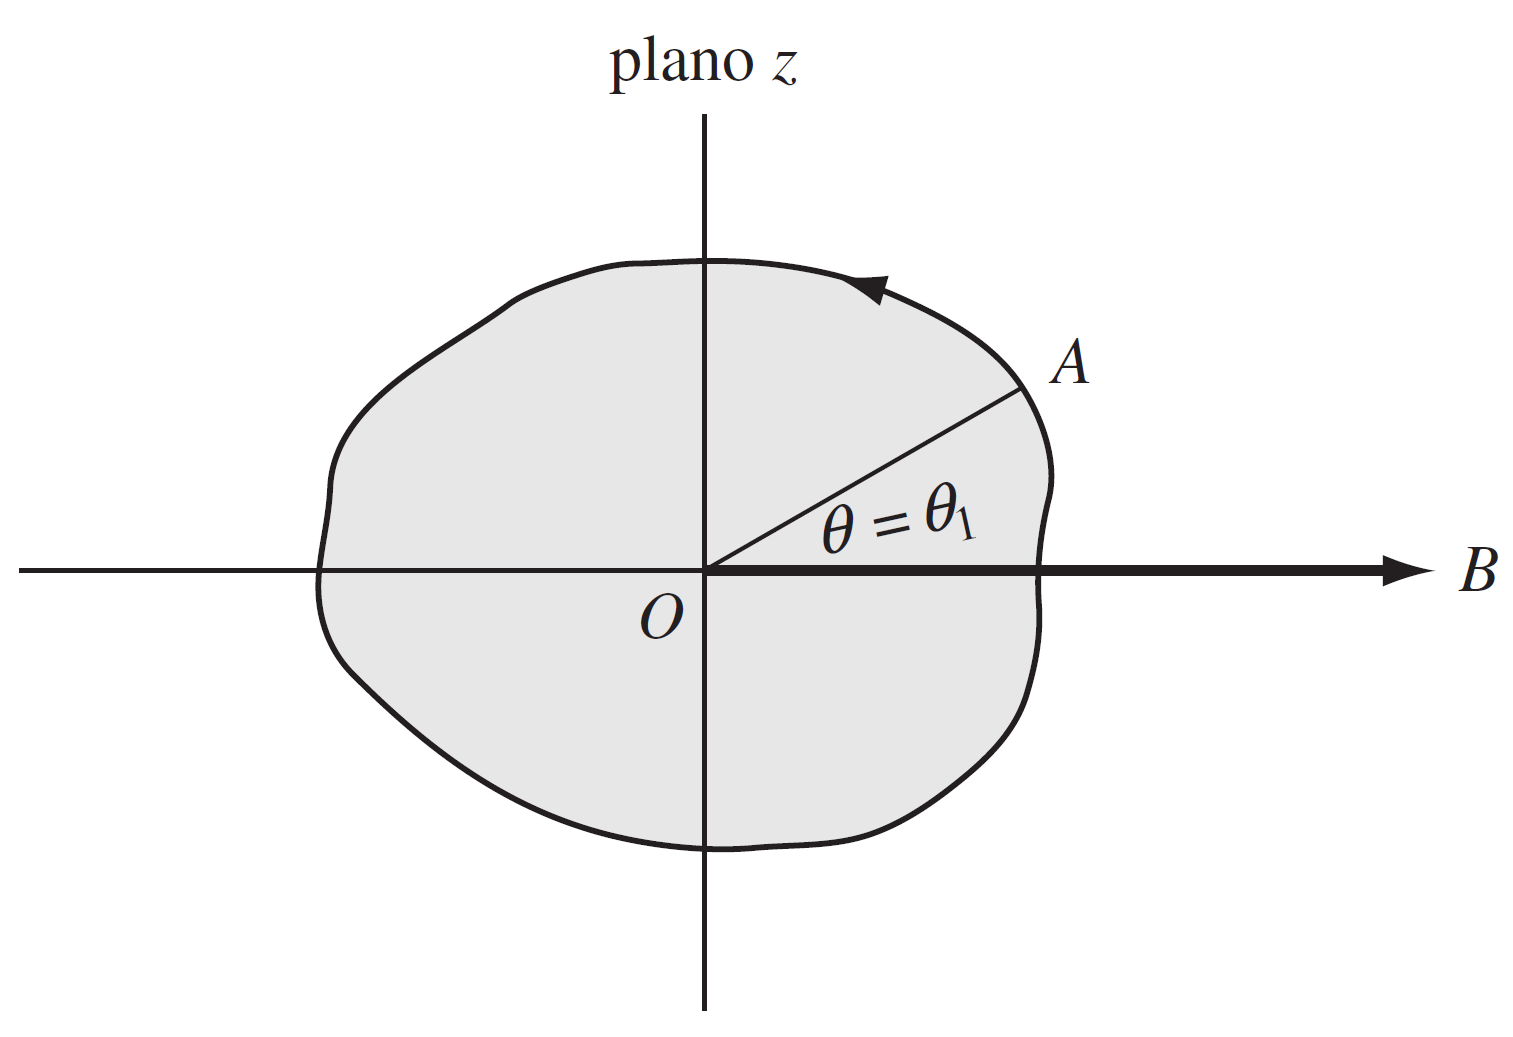
\includegraphics[scale=0.3]{ramificaciones.png}
\caption{Ejemplo de ramificación}
\end{figure}



\section{Superficies de Riemann} 

Existe una manera análoga de lograr lo mismo que con la línea de ramificación. Para esto debemos imaginarnos el plano $z$ como dos capas superpuestas, ambas cortadas por la recta $OB$, y que el borde inferior de la capa inferior se une con el borde superior de la capa superior, de tal modo que si se continúa dando vueltas se va de la capa superior a la capa inferior y así recurrentemente. \\

El caso de dos capas corresponden a la función $z^{1/2}$, pero evidentemente puede haber mas superficies de Riemann con mas capas. El conjunto de todas las capas hace la \textit{superficie de Riemann}. Por ejemplo para la función $w = \ln z$ existen infinitas capas.

\section{Límites y continuidad}

\subsection{Limites}

Los límites se definen de manera análoga a como se hace en el caso real, o de $\mathbb{R}^n$. Decimos que A es el límite de $f(z)$ tendiendo a $z_0$ como:

\begin{equation}
\lim_{z \rightarrow z_0} f(z)  = A  \ \ \mathrm{si} \ \forall \ \epsilon > 0, \ \epsilon \in \mathbb{R} \  \exists \ \delta \ / \ A - f(z) < \epsilon   \ \forall \ z \ \mathrm{tal \ que} \ z-z_0 < \delta
 \end{equation}

Cuando estamos en funciones multivaluadas en general el límite depende de en que rama nos encontremos. Además mucho de los teoremas sobre límites para funciones reales son válidos para funciones complejas, tales como:

\begin{equation}
\lim_{z \rightarrow z_0} (f(z)+g(z)) = \lim_{z \rightarrow z_0} f(z) + \lim_{z \rightarrow z_0} g(z)
\end{equation}

\begin{equation}
\lim_{z \rightarrow z_0} (f(z) g(z)) = \ccorchetes{\lim_{z \rightarrow z_0} f(z)} \cdot \ccorchetes{\lim_{z \rightarrow z_0} g(z) }
\end{equation}

\begin{equation}
\lim_{z \rightarrow z_0}  \dfrac{f(z)}{g(z)} = \dfrac{\lim_{z \rightarrow z_0}  f(z)}{\lim_{z \rightarrow z_0} g(z)} \ \mathrm{si} \ \lim_{z \rightarrow z_0} g(z) \neq 0
\end{equation}



\shadowbox{\textbf{Ejemplo 2.3}}

\hrulefill

Vamos a demostrar que el limite  $\lim_{z \rightarrow 0} \bar{z}/z$ no existe. \\

Si existiera el límite está claro que da igual el camino escogido para llegar al punto 0, debe dar igual que dirección cojamos al aproximarnos. Entonces estudiaremos la mas básica. Si $z=x+iy$, una condición para que exista límite: 

\begin{equation}
\lim_{x \rightarrow 0} \lim_{y \rightarrow 0} f(z) = \lim_{y \rightarrow 0} \lim_{x \rightarrow 0} f(z)
\end{equation}

Si ahora comprobamos eso para la función $\frac{x-iy}{x+iy}=f(z)$:

$$ \lim_{x \rightarrow 0} \lim_{y \rightarrow 0} \frac{x-iy}{x+iy} = \lim_{x \rightarrow 0} \dfrac{x}{x} = 1 $$

$$ \lim_{y \rightarrow 0} \lim_{x \rightarrow 0} \frac{x-iy}{x+iy} =  \lim_{y \rightarrow 0} \frac{-iy}{iy} = -1 $$

\hrulefill \\


\subsection*{Continuidad}

Decimos que una función $f(z)$ es \textit{continua} en $z=z_0$ si:

\begin{itemize}
\item $f(z_0)$ esta univocamente definida cuando $z=z_0$

\item $\lim_{z \rightarrow z_0} f(z) = f(z_0)$
\end{itemize} 

\begin{theorem}
 una función $f(z)$ es continua en $z=z_0$ si y solo si sus partes reales e imaginaras $w(x,y)$ y $v(x,y)$ son funciones continuas de $x$ e $y$ en $(x_0,y_0)$
\end{theorem}

\section{Diferenciabilidad}

Sea $f(z)$ una función univoca en alguna región $R$ del plano $z$, decimos que $f(z)$ es \textit{diferenciable} si existe el límite:

\begin{equation}
\derivadas{f}{z} = f'(z) = \lim_{\Delta z \rightarrow 0} \frac{f(z+\Delta z)-f(z)}{\Delta z}
\end{equation}

Si la derivada existe en todo punto de una región diremos entonces que $f(z)$ es \textit{analítica} en $R$. A veces a una función analítica se le llamada función \textit{holomorfa} o \textit{regular}. \\


\begin{definicion}
una \textbf{función holomorfa} es una función compleja que es diferenciable en cada punto de un dominio abierto en el plano complejo. En otras palabras, una función f(z) es holomorfa si la derivada f'(z) existe en cada punto z del dominio abierto. 
\end{definicion}

La propiedad clave de las funciones holomorfas es que son analíticas, lo que significa que pueden ser representadas por una serie de potencias convergente en todo su dominio


Esta definición es formalmente idéntica a la definición de derivada y condición de derivavilidad de una función en variable real, por lo que todas las reglas del producto, cociente, cadena ... son aplicables también a las funciones de variable compleja. \\

En el caso de hablar de funciones multivaludas (como la logarítica) nos referiremos a una rama en concreto. Por ejemplo la rama principal del logaritmo. \\


Ahora nos vamos a preguntar cuales son las condiciones para que una función sea diferenciable sin tener que estudiar en todo punto el límite. Entonces nos preguntamos: ¿Existe alguna condición suficiente para demostrar la diferenciabilidad de una función en $R$? De aquí nace el siguiente teorema: \\

\begin{theorem}
Sea la función $f(z)=u+iv$ analítica en una región $R$. Entonces se verificarán las \textbf{ecuaciones de Cauchy-Riemann}, que son:
$$ \parciales{u}{x} \ = \ \parciales{v}{y}  $$
$$ \parciales{u}{y} \ = - \parciales{v}{x} $$
\end{theorem}

Ahora bien, ¿Que una función verifique las ecuaciones de Cauchy-Riemann implica  que la función es analítica? La respuesta, en general, es que no. Sin embargo solo hace falta añadirle a estas ecuaciones una pequeña condición para que se verifiquen: que tanto $u(x,y)$ como $v(x,y)$ sean continuas en sus primeras derivadas. Si se verifica esto y las ecuaciones de Cauchy-Riemann, una función es analítica. \\

Otra forma de escribir las ecuaciones de Cauchy-Riemann es:

\begin{equation}
\parciales{f(z)}{\bar{z}}=0
\end{equation}

\begin{theorem}
Si $f(z)$ es analítica en una región $R$ entonces todas sus derivadas de orden superior existen en $R$
\end{theorem}


\section{Singularidades}

Un punto en el que una función $f(z)$ deja de ser analítica se denomina \textit{punto singular} o \textit{singularidad} de $f(z)$. Existen varios tipos de singularidades, muy relevantes para el tema 3.

\begin{itemize}
\item \textbf{Singularidad aislada:} se denomina así a los puntos tales que $\exists \gamma >0 $ tal que en la región $|z-z_0|$ no existe otro punto singular. Si no existe tal $\gamma$ se dice que es una singularidad no aislada.

\item \textbf{Polos:} si $z_0$ es una singularidad tal que $f(z)$ tal que se puede encontrar un entero positivo tal que:

\begin{equation}
\lim_{z \rightarrow z_0} (z-z_0)^n f(z) \neq 0
\end{equation}

se dice que $z=z_0$ es un \textit{polo de orden n}. Llamamos \textit{polo simple} si $n=1$. En general las funciones con polos se suelen comportar como:

\begin{equation}
f(z) \thicksim \frac{C}{(z-z_0)^n}
\end{equation}


en el entorno del polo. De manera análoga decimos que la función $g(z)$ tiene un \textit{cero de orden n} en $z_0$ si $f(z)=(z-z_0)^{-n} g(z)$ tal que $f(z_0) \neq  0$. 

\item \textbf{Puntos de ramificación:} una función multivoca no es continua en el punto de ramificación, ya que el límite depende de la dirección, y por tanto tampoco es anaítica.

\item \textbf{Singularidad evitable:} se le llama así a un punto que no es analítico pero en el que si existe límite.

\item \textbf{Singularidad esencial:} se le llama  así a un punto singular que no sea ni un polo, ni punto de ramificación ni singularidad evitable. Un ejemplo es el punto $z=0$ para la función $f(z)=e^{1/z}$.
\end{itemize}

\chapter{Integral compleja}

\section{Curva de Jordan}

Se define como \textit{arco} a la parametrización continua:

\begin{equation}
z=z(t) \quad t_1 \leq t \leq t_2
\end{equation}

si $t_1 = t_2$ se dice que el arco es una \textit{curva cerrada}.  \\

Un \textit{arco de Jordan} es aquel arco que no se corte a si mismo:

\begin{equation}
\forall t,t^* \in [t_1,t_2), t\neq t^* \Longrightarrow z(t)\neq z(t^*)
\end{equation}

siendo la \textit{curva de Jordan} aquella curva cerrada que no se corte a si misma.

\section{Integral de línea}

Sea $C$ una curva regular en todo punto, definimos como \textit{integral de línea} al límite:

\begin{equation}
lim_{n \rightarrow \infty} \sum_{i=1}^n f( \xi_k) \Delta z_k
\end{equation}

siendo $\xi_k$ un punto cualquiera en el intervalo $(z_{k-1},z_k)$ y $\Delta z_k = z_k-z_{k-1}$.  Cuando $n \rightarrow \infty$ este $\Delta z_k \rightarrow 0$. \\

Al igual que con las derivadas la integral de línea compleja se define de la misma manera que una integral en variable real, por lo que muchas de sus propiedades son análogas. \\

\section{Teorema fundamental del cálculo}

Definimos como \textit{función primitiva} de $f(z)$ a una función $F(z)$ tal que:

\begin{equation}
F'(z) = f(z)
\end{equation}

también se le suele llamar \textit{integral indefinida} ya que:

\begin{equation}
F(z) = \int f(z) \D z
\end{equation}

\begin{theorem}[teorema fundamental del cálculo] 
sea la curva $C$ una curva que une los puntos $a$ y $b$; y $F(z)$ la primitiva de la función integrable $f(z)$, tenemos que:

$$ \int_C f(z) \D z = F(b) - F(a) $$

\end{theorem}

Por lo tanto queda claro que si una función es integrable en $R$, da igual que curva elijamos para unir un punto a otro, el resultado será el mismo. En otras palabras: la integral es independiente del camino. Si la integral se hiciese a lo largo de una curva cerrada queda claro que la integral sería 0. Este resultado es equivalente: si una función continua a lo largo de una integral cerrada es cero, también es integrable. \\ %Demostrar esto

\section{Teorema de Cauchy}

Antes de continuar vamos a introducir dos pequeñas definiciónes: 

\begin{itemize}
\item \textbf{Región simplemente conexa:} llamamos a la región $R$ \textit{simplemente conexa} si cualquier curva cerrada contenida en $R$ se puede contraer continuamente a un punto $R$ sin salirnos de $R$. De manera poco rigurosa se podría decir que si la función no tiene agujeros en ningún punto la función es simplemente conexa. %poner un dibujo \\ 

\item \textbf{Subconjunto convexo:} decimos que un subconjunto de $R$ del plano es \textit{convexo} si para cualquiera dos puntos $z_1$ y $z_2$ de $R$ el segmento que los une está contenido en $R$. Es decir, si somos capaz de trazar una recta entre $z_1$ y $z_2$ sin que se salga de $R$, decimos que dicha recta es un subconjunto convexo. %dibujo

\item \textbf{Homótopo.} Supóngase las curvas $C$ y $C'$. Si somos capaces de obtener $C'$ a partir de $C$ a partir de un número finito de deformaciones elementales se dice que $C$ es homótopo a $C'$, y se expresa como: $C \thicksim C$.  %dibujo

\end{itemize}

Existe otra manera de definir una región simplemente conexa que implica definir un camino \textit{nul-homotopo}. Llamamos \textit{camino nulo} a las curvas tal qeu $z(t) = a$. Si un camino es homotopo a un camino nulo, tenemos que dicho camino es \textit{nul-homotopo}. Una región es simplemente conexa si todo camino cerrado es nul-homotopo. \\

Cauchy fue capaz de demostrar que si  $f(z)$ es una función analítica en una región $R$, $f(z)$ es integrable en $R$, enunciando así el siguiente teorema:

\begin{theorem}[teorema de Cauchy]
sea $f(z)$ una función analítica en una región simplemente conexa $R$. Entonces si $C$ es una curva cerrada arbitraria contenida en $R$, se verifica que:

$$ \oint_C f(z) \D z = 0 $$
\end{theorem}

Sin embargo existen formas de demostrar que el teorema de Cauchy se puede ampliar más, ya que funciona para cualquier subconjunto de $R$ convexo sin que $R$ sea una región simplemente conexa. \\


En muchas ocasiones hacemos integrales de contorno en una región abierta $R$ limitada por una curva de Jordan $C$. Si la función que queremos integrar en $C$ es analítica en el interior de la curva y continua en el contorno (continua en $C$) el teorema de Cauchy es válido para $C$.  \\


Ahora, supongamos que la región $R$ donde $f(z)$ es analítica está limitada por dos curvas cerradas de Jordan $C$ y $C_1$ tal que:  \\ % dibujo

Entonces tenemos que:

\begin{equation}
\oint_c f(z) \D z = \oint_{C_1} f(z) \D z 
\end{equation}

La interpretación de este resultado es que podemos mover el contorno $C$ hasta convertirlo en el contorno $C_1$ (mediante deformaciones elementales, ya que no hay puntos singulares en $R$), de tal manera que se pueda recorrer la siguiente curva: %dibujo \\


Entonces este resultado, hecho así, es trivial, teniendo en cuenta que si cambiamos el sentido de giro cambia el signo. Entonces podemos hacer la analogía con $n$ curvas de Jordan obteniendo que:

\begin{equation}
\oint_C f(z) = \oint_{C_1} f(z) \D z + \ldots \oint_{C_n} f(z) \D z 
\end{equation}

Es muy importante saber que se define como sentido positivo del recorrido aquel que deja la región a la izquierda del giro (en general, sentido anti-horario); por lo que la anterior de ecuación se verifica cuando todas las curvas se hacen con el mismo sentido de giro. \\

\shadowbox{\textbf{Ejemplo 3.1}}

\hrulefill

Vamos a calcular las integrales de Fresnel usando el teorema de Cauchy:

\begin{equation}
\int_{0}^{\infty} \cos (x^2) \D x = M \tquad 
\int_{0}^{\infty} \sin (x^2) \D x = N
\end{equation}


Igualamos a los valores $M$ y $N$ para no repetir posteriormente de manera constante la expresión de las integrales. Para esto vamos a hacer la integral de la función $f(z)=e^{iz^2}$ en el siguiente entorno:

\begin{figure}[h!] \centering
\begin{tikzpicture}
\draw[step=1cm,gray,ultra thin] (0,0) grid (3,3);
\draw[->] (-.2,0) -- (3.2,0);
\draw[thick,->] (0,0) -- (3,0);
\draw[->] (0,-.2) -- (0,3.2);
\draw[thick,->] (2.121320343559643,2.121320343559643) -- (0,0) ;
\draw[thick,->] (3,0) arc [start angle=0, end angle=45, radius=3];  
\draw[ultra thin] (1.5,0) node[below] {$Re$};
\draw[ultra thin] (0,1.5) node[left] {$Im$};
\draw[ultra thin] (2.121320343559643,2.121320343559643) node[above] {$B$};
\draw[ultra thin] (3.2,0) node[right] {$A$};  
\draw[ultra thin] (0,-0.2) node[below] {$O$};
\end{tikzpicture}
\end{figure}

Entonces por el teorema de Cauchy la integral cerrada de la curva $C$ será 0. A su vez esta podemos dividirla en 3 trozos, por lo que:

$$ \int_{OA} f(z) \D z +  \int_{AB} f(z) \D z +  \int_{BO} f(z) \D z = 0  $$

Y cada una de estas integrales tienen diferente forma, ya que $z$ adoptará formas diferentes. Entonces:

\begin{itemize}
\item La integral de $OA$ se hace en el plano real, por lo que $z = x$, y integramos desde $x \in (0,R$).
\item La integral de $AB$ se integra en un arco, por lo que $z=Re^{i \theta}$ , integrando el ángulo entre $\theta \in (0, \pi/4$).
\item La integral de $BO$ se integra en la recta $z = x + iy$ o lo que es lo mismo $z=re^{i (\pi/4)}$, con $r \in (0,R)$.
\end{itemize}

Hagamos cada una de estas integrales por separado. Tenemos que:

\begin{itemize}
\item Integral $OA$. Tenemos que $f(z) = e^{ix^2} = \cos (x^2) + i \sin (x^2)$, como $z = x$, $\D z = \D z$, por lo que tenemos que la integral:

$$ \int_{OA} f(z) \D z = \int_{0}^{R} (\cos (x^2) + i \sin (x^2)) \D x   $$

que si $R \rightarrow \infty$ tenemos que:

$$ \int_{OA} f(z) = M + iN  $$

\item Integral $BO$. Tenemos que $f(z) = e^{i r^2 e^{i \pi/2}} = e^{-r^2}$, y además $\D z = e^{\pi/4}  \D r = \frac{(1+i)}{\sqrt{2}} \D r$. Entonces es fácil de deducir que:

$$ \int_{BO} f(z)\D z = \int_R^0 e^{\pi/4} e^{-r^2} \D r = - \dfrac{(1+i)}{\sqrt{2}} \dfrac{1}{2} \sqrt{\pi(1-e^{-R^2})} $$

que si $R \rightarrow \infty$ tenemos que:

$$ \int_{BO} f(z)\D z  =  -  \parentesis{\dfrac{\pi}{2^3}}^{1/2}   \parentesis{1 + i}  $$

Donde hemos asumido que la integral:

$$ \into e^{-r^2} \D r = \dfrac{\sqrt{\pi}}{2}  $$

que es la integral gaussiana. Es muy fácil de deducir ya que si llamamos I al resultado, y usando luego el cambio a polares (e integrando en un cuarto del plano):

$$ I^2 = \into  \into e^{-x^2} e^{-y^2} \D x \D y = \int_{0}^{\pi/2} e^{-r^2} r \D r \D \theta = \dfrac{\pi}{2} \parentesis{\dfrac{1}{2} e^{-r{^2}}}_{0}^\infty = - \dfrac{\pi}{4} $$

\item Integral $AB$. Esta integral tiende trivialmente a cero cuando $R \rightarrow \infty$. Para demostrarlo acotaremos la integral a una expresión tal que cuando $R \rightarrow 0$ tienda a cero, y por lo tanto por estar acotado por esto la integral también tenderá a cero:

$$ \int_{AB} f(z) \D z = \int e^{i R^2 e^{i 2 \theta}} R e^{i \theta} i \D \theta = \int e^{i (R^2 (cos (2 \theta) + i \sin (2 \theta))+\theta)} R i \D \theta  $$

Ahora comenzamos a acotar. Antes vamos a introducir unas pequeñas simplificaciones que vamos a usar. Es evidente que $|i|=1$, que $|e^{i f(x)}| = 1$ si $f(x)$ es una función de variable real (se puede expresar en función de senos y cosenos, el módulo complejo nunca saldrá del circulo $R = 1$). Entonces:

$$ \left| \int f(z) \D z \right| \leq \int \left| f(z) \D z \right| = \int_{0}^{\pi/4} \left| e^{i(R^2 \cos ( 2 \theta) + \theta)}  \right| \left| e^{-i R^2 \sin(2 \theta)} \right| |R||i||\D \theta| = \int_0^{\pi/4} R \left| e^{-R^2 \sin 2 \theta} \right| \D \theta $$

Como sabemos que $\sin \theta  \geq \frac{2 \cdot \theta}{\pi}$ si $\theta \in [0,\pi/2]$, si hiceramos el cambio $2 \theta = \varphi$, tendríamos que:

$$ \int_0^{\pi/4} R \left| e^{-R^2 \sin 2 \theta} \right| \D \theta \leq \frac{R}{2} \int_0^{\pi/2} e^{-R^2 \frac{\varphi}{\pi}} \D \varphi = \dfrac{1}{2 \pi} \dfrac{1}{R} (e^{-R^2/2}-1)   $$

Que por lo tanto si $R \rightarrow \infty$ tenemos que:

$$ \int_{AB} f(z) \D z \rightarrow 0 $$


\end{itemize}

Si $R \rightarrow \infty$ en la suma de las integrales es sencillo de ver que:

$$ M + i N - (1+i)\sqrt{\dfrac{\pi}{2^3}} = 0  $$

Lo que nos lleva a deducir directamente que:

\begin{equation}
\into \cos (x^2) \D x = \dfrac{\sqrt{\pi}}{2 \sqrt{2}}
\end{equation}

\begin{equation}
\into \sin (x^2) \D x = \dfrac{\sqrt{\pi}}{2 \sqrt{2}}
\end{equation}


\hrulefill \\


\chapter{Integrales de Cauchy}

\section{Formula integral de Cauchy}

Supongamos $f(z)$ analítica en una región $R$ simplemente conexa y que es continua sobre $C$ (de tal forma que verifica el teorema de Cauchy). Si $C$ es una curva de Jordan recorrida en el sentido positivo, sea $a$ un punto arbitrario en el interior de la $C$, tenemos que: 

\begin{equation}
f(a) =  \frac{1}{2 \pi i} \oint_C \frac{f(z)}{z-a} \D z
\end{equation}

que es la denominada \textbf{fórmula integral de Cauchy}. Es una fórmula muy poderosa, ya que implica determinar el valor de una función analítica en una región conociendo solo los valores de la frontera. \\


\shadowbox{\textbf{Ejemplo 4.1}}

\hrulefill

Vamos a calcular la siguiente integral de linea usando de manera sencilla la fórmula integral de Cauchy:

\begin{equation}
\oint_C  \frac{\sin \pi z^2 + \cos \pi z^2}{(z-1)(z-2)} \D z
\end{equation}

a través de la circunferencia $|z| = 3$. Esta claro que para aplicar la fórmula integral de Cauchy primero vamos a tener que separar la división entre dos divisores a una suma de dos divisiones. Podemos ver que:

$$ \dfrac{f(z)}{(z-1)(z_2)} = \dfrac{f(z)}{z-2} - \dfrac{f(z)}{z-1} $$


entonces podemos ver que la integral:

$$  
\oint_C  \frac{\sin \pi z^2 + \cos \pi z^2}{(z-1)(z-2)} \D z  = 
\oint_C  \frac{\sin \pi z^2 + \cos \pi z^2}{z-2} \D z + 
\oint_C  \frac{\sin \pi z^2 + \cos \pi z^2}{z-1} \D z  = $$

$$ = 2 \pi i (\sin 4\pi + \cos 4\pi) - 2 \pi i (\sin \pi + \cos \pi) = 4 \pi i  $$

\hrulefill \\

\subsection{Teorema de Taylor}

\begin{theorem}[Teorema de taylor]
sea $f(z)$ analítica dentro y sobre una curva de Jordan $C$. Sea $a$ un punto del a región $R$ interior a $C$. Entonces, en un entorno centrado en $a$, $f(z)$ se puede representar como:

$$ f(z) = f(a) + f'(a)(z-a)+f''(a) \dfrac{(z-a)^2}{2!} + \ldots = \sum_{n=0}^\infty \frac{f^{(n)}(a)}{n!} (z-a)^n $$
\end{theorem}


Esta serie de potencias se llama serie de Taylor y converge en un disco abierto a $|z-a|<r$ donde $r$ es la distancia del punto $a$ a su singularidad más próxima. Una de las implicaciones de este teorema es una propiedad muy potente, que dice lo siguiente:

\begin{theorem}
si $f(z)$ es analítica en una región $R$, entonces todas las derivadas de $f(z)$ son analíticas en $R$, es decir todas sus derivadas existen en $R$. 
\end{theorem}


\subsection{Fórmula integral de Cauchy para las derivadas}

De la formula integral de Cauchy se puede hacer para las derivadas usando las series de taylor, de tal manera que:


\begin{theorem}
sea $f(z)$ una función analítica en una región simplemente conexa $R$ y continua sobre su frontera $C$. Sea $C$ una curva cerrada de Jordan y $a$ un punto del interior de $C$. Se verifican entonces las fórmulas integrales de Cauchy:

$$ f^{(n)} (a) = \frac{n!}{2 \pi i} \int \frac{f(w)}{(w-a)^{n+1}} \D w $$
\end{theorem}


Entonces el resultado de la fórmula integral de Cauchy es mucho mas poderoso del que era inicialmente: no solo te permite calcular la derivada en un punto conociendo los valores de la función en el contorno, si no que incluso te permite calcular los valores de cualquier derivada en cualquier punto del conjunto $R$.  

\subsection{Fórmula integral de Cauchy para curvas nul-homotopas}

Vamos a introducir un teorema que amplíe ka fórmula integral de cauchy para curvas que se corten, dando varias vueltas al mismo punto:

\begin{theorem}
sea $f(z)$ una función analítica en una región $R$. Sea $C$ una curva cerrada nul-homotopa contenida en $R$ y sea $a$ un punt ode $R$ que no pertenece a $C$. Entonces si la curva $C$ da $n(C,a)$ vueltas al punto $a$, tenemos que:
$$ n(C,a) f(a) = \frac{1}{2 \pi i} \oint_C \frac{f(z)}{z-a} \D z $$
\end{theorem}

De hecho es muy fácil comprobar que este teorema se reduce a la primera fórmula integral de Cauchy que hemos dado si solo damos una vuelta en sentido anti-horario al punto $a$.

\section{Residuo}

Definimos \textbf{residuo} de la función $f(z)$ en el polo de orden $n$ $z=a$ a la siguiente expresión:

\begin{equation}
\Res (f;a) = \lim_{z \rightarrow a} \ccorchetes{\dfrac{1}{(n-1)!} \dfrac{\D^{n-1}}{\D z^{n-1}} \parentesis{(z-a)^n f(z)}}
\end{equation}

Vamos a enunciar ahora un teorema que es consecuencia directa de las fórmulas integrales de Cauchy:

\begin{theorem}[teorema del residuo]
Sea $f(z)$ una función analítica en el interior y sobre una curva cerrada de Jordan $C$ excepto en un número finito de puntos $a_1,\ldots,a_n$ en los cuales $f(z)$ tiene polos de orden $n_1,\ldots,n_N$. Entonces:
$$ \oint_C f(z) \D z = 2 \pi i \sum_{j=1}^N \Res (f;a_j) $$
\end{theorem}

El teorema del residuo nos permite calcular integrales a lo largo de caminos cerrados que contienen polos. En ese caso el cálculo de una integral se reduce al cálculo de los residuos, que se resuelven derivando y haciendo límites. Si no hay singularidades en el interior (es decir es analítica en todo $R$) tenemos que la suma de los residuos es cero verificándose el teorema de Cauchy. En el tema siguiente veremos un teorema (teorema de Laurent) que incluya todos las singularidades, tales como putos de ramificación... \\



\shadowbox{\textbf{Ejemplo 4.2}}

\hrulefill

Sea $C$ el círculo $z=4$. Calculemos:

\begin{equation}
\oint  \frac{e^z}{(z^2+\pi^2)^2} \D z
\end{equation}

Tenemos que $1/(z^2+\pi^2) = 1/((z+i\pi)(z-i \pi))$. Entonces tenemos dos polos de orden 2 en $+i$ y $-i$. Por lo tanto tenemos que calcular ambos residuos:

\begin{itemize}
\item Residuo $+i$. Aplicamos la fórmula:

$$ \lim_{z \rightarrow i\pi} \dfrac{\D}{\D z} \parentesis{\dfrac{e^z (z- i \pi)^2}{(z+i \pi)^2 (z - i \pi)^2 }} = \lim_{z \rightarrow i\pi} \parentesis{\dfrac{e^z}{(z+i \pi)^2 }- \dfrac{2 \cdot e^z}{(z+i \pi)^3 } }= \dfrac{-1}{-4 \pi^2}- \dfrac{-2}{- 8 \pi^3 i} $$

\item Residuo $+-$. Aplicamos la fórmula:

$$ \lim_{z \rightarrow -i\pi} \dfrac{\D}{\D z} \parentesis{\dfrac{e^z (z+ i \pi)^2}{(z+i \pi)^2 (z - i \pi)^2 }} = \lim_{z \rightarrow i\pi} \parentesis{\dfrac{e^z}{(z-i \pi)^2 }- \dfrac{2 \cdot e^z}{(z-i \pi)^3 } }= \dfrac{-1}{-4 \pi^2}- \dfrac{-2}{8 \pi^3 i} $$
\end{itemize}

Entonces tenemos que la suma de ambos residuos:

$$ \Res (f(z),i \pi) + \Res (f(z), - i \pi) = \dfrac{2}{4\pi^2}$$

Y por lo tanto:


\begin{equation}
\oint  \frac{e^z}{(z^2+\pi^2)^2} \D z = \dfrac{i}{\pi}
\end{equation}

\hrulefill \\


Ahora vamos a introducir un teorema sumamente útil que facilitará el cálculo de integrales definidas en variable real. 

\begin{theorem}
sea $\Gamma$ un arco del circulo $|z|=R$ y sea $f(z)$ una función que para $R$ suficientemente grande satisface:

$$ f(z) \leq \frac{M}{R^k} $$

tal que $z=Re^{i \theta}$, donde $M>0$ y $k>1$. Entonces:

$$ \lim_{R \rightarrow \infty} \int_{\Gamma} f(z) \D z = 0 $$

\end{theorem}

Este procedimiento se suele usar para las funciones racionales, ya que es muy fácil demostrar la condición de $f(z) \leq M/R^k$.

\section{Teorema de Morera}

Sabemos que el teorema de Cauchy nos dice que una función analítica en una región $R$ simplemente conexa cumplirá que cualquier integral cerrada en $C$ contenida en $R$ es cero. El teorema de Morera demuestra el recíproco:

\begin{theorem}[teorema de Morera]
sea $f(z)$ una función continua en una región $R$ simplemente conexa. Si para toda curva cerrada $C$ contenida en $R$ se verifica que: 
$$ \oint_C f(z) \D z = 0 $$
entonces $f(z)$ es analítica en $R$.
\end{theorem}

\section{Desigualdad de Cauchy y Teorema de Liouville}

Otro resultado que es consecuencia de las fórmulas integrales de Cauchy es:

\begin{theorem}[desigualdad de Cauchy]
si $f(z)$ es analítica dentro y sobre un círculo $C$ de radio $r$ y centro $z=a$, entonces:
$$ \left|  f^{(n)}(a) \right| \leq \frac{M(r) n!}{r^n}$$
en donde $M(r)$ es una constante real y positiva tal que $|f(z)|<M(r)$. Es decir, $M(r)$ es una cota superior de $|f(z)|$ sobre $C$. Escribimos que depende de $r$ porque para cada círculo existirá una cota diferente. Una vez que hemos dado un radio podremos definir la cota, no antes.
\end{theorem}

Un resultado directo de la desigualdad de Cauchy es:

\begin{theorem}[teorema de Liouville]
Supongamos que para todo $z \in C$ la función $f(z)$ satisface las dos condiciones siguientes:

\begin{itemize}
\item $f(z)$ es analítica 
\item $f(z)$ es acotada, es decir:   $\exists \ M > 0 \ \ / \ \ |f(z)|<M  \  \forall  \ z \in C$
\end{itemize}
Entonces $f(z)$ debe ser una constante

\end{theorem}

\section{Teoremas}

\subsection{Teorema fundamental del álgebra}

Una consecuencia importante y directa del teorema de Liouville es el teorema fundamental del álgebra (que como su propio nombre indica es muy relevante, además de poderoso).

\begin{theorem}[teorema fundamental del álgebra]
Sea $P(z) = a_0+a_1 z+ \ldots+ a_n z^n $ un polinomio no constante ($n \geq 1, a_n \neq 0$). Entonces la ecuación $P(z)=0$ tiene al menos una raíz compleja.
\end{theorem}

es un argumento poderosísimo que solo se puede entender en variable compleja. En variable real resulta imposible demostrar algo así, ya que hay polinomios que  no tienen solución. De hecho este teorema tiene un corolario que muchas veces se usa como el propio teorema fundamental del algebra. Este es:

\begin{corollary}
la ecuación polinómica 
$$ P(z) = a_0 +a_1 z + a_2 z^2 + \ldots + a_n z^n = 0 $$
tiene exactamente $n$ raices, teniendo en cuenta la multiplicidad. 
\end{corollary}


\subsection{Teorema del argumento}

El teorema del argumento nos permite conocer el número de polos y ceros encerrados en el interior de una curva, lo cual es muy útil, ya que podremos ir acotando estos valores para funciones muy complicadas.

\begin{theorem}[teorema del argumento]
sea $f(z)$ una función analítica en el interior de y sobre una curva cerrada de Jordan $C$ positivamente orientada, excepto en un número finito de polos en el interior $C$. Entonces:

$$ \frac{1}{2 \pi i} \oint_C \frac{f'(z)}{f(z)} \D z = N - P $$

siendo N el número de ceros y P el número de polos de $f(z)$ encerrados en la curva $C$, contando multiplicidades (un polo de orden dos cuenta como P=2)
\end{theorem}


El teorema del argumento nos permite estudiar cuanto varía el argumento de una función al recorrer un camino cerrado de sentido anti-horario. La diferencia entre el número de ceros y de polos comprendidos en el interior de una curva cerrada $C$ es igual a la variación de $\Arg f(z) / 2 \pi$ al recorrer la curva $C$ en la dirección contraria a las agujas del reloj. 



\subsection{Teorema de Rouche}

El teorema de Rouche nos permite acotar de otra forma el número de ceros (contando las multiplicidades) de una función. 

\begin{theorem}[teorema de Rouche]
sean $f(z)$ y $g(z)$ dos funciones analíticas en el interior y sobre una curva de Jordan simple $C$. Si $|f(z)|>|g(z)|$ en todo punto de $C$, entonces las funciones $f(z)$ y $f(z)+g(z)$ tienen el mismo número de ceros, contando sus multiplicidades en el interior de $C$.
\end{theorem}

Vamos a ver un ejemplo para localizar los ceros de polinomios en ciertas regiones del plano complejo:\\

\shadowbox{\textbf{Ejemplo 4.3}}

\hrulefill

Vamos a calcular cuantos ceros tiene el polinomio siguiente de modulo menor que 1:

$$ P(z) = z^8 - 4z^5 + z^2 - 1 $$

En la circunferencia de radio 1 $z=Re^{i\theta} \ / \ R=1$, por lo que $|z|=1$. Está claro que si $f(z) = - 4 z^5$ llegamos a $|f(z)| = 4$. Y la función $g(z) = z^8 + z^2 -1$ cumplirá que $|g(z)|=3$. Por el teorema de Rouche $f(z)+g(z)$ tendrá el mismo número de ceros que $f(z)$ en dicho círculo. Entonces el polinomio $P(z)$ tendrá 5 ceros en el interior del círculo. 


\hrulefill \\



\subsection{Teorema del valor medio de Gauss}

En algunas asignaturas tales como Electromagnetismo I o Métodos V hemos estudiado el teorema del valor medio de Gauss, que nos permite conocer el promedio de los valores sobre una circunferencia de una función conociendo un valor en el centro de la circunferencia. Mientras que para aplicar este teorema en variable real hace falta que la función sea armónica, en variable compleja es mucho menos restrictivo.

\begin{theorem}[teorema del valor medio de Gauss]
sea $f(z)$ analítica dentro y sobre un círculo $C$ con centro en $a$ y radio $r$, entonces $f(a)$ es el promedio de los valores de $f(z)$ sobre $C$, es decir:

$$ f(a) = \frac{1}{2 \pi} \int_0^{2\pi} f(a+re^{i \theta}) \D  \theta $$
\end{theorem}

Del que directamente se puede deducir el siguiente lema:

\begin{lemma}
Sea $f(z)$ analítica en un disco abierto centrado en $z=a$ y de radio $r$: 

$$ B(a,r) = \{ z \in C / |z-a|<r \} $$

si $|f(z)|\leq|f(a)|$ para todo $z \in B$, entonces $f(z)$ tiene el valor constante $f(a)$ en todo $B(a;r)$.
\end{lemma}

\subsection{Teorema del módulo máximo y mínimo}

Tanto teorema del módulo máximo como el del módulo mínimo son deducciones directas del teorema del valor medio de Gauss y su lema.
 
\begin{theorem}[teorema del módulo máximo]
sea $f$ una función continua en una  región acotada $R$ y en su frontera. Supongamos que $f(z)$ es analítica y no constante en el interior de $R$. Entonces el valor máximo de  $|f(z)|$ se alcanza siempre y ocurre en algún punto de la frontera de $R$, nunca en su interior.
\end{theorem}

\begin{theorem}[teorema del módulo mínimo]
sea $f(z)$ una función continua en una región acotada $R$ y en su frontera. Supongase que $f(z)$ es analítica, no constante y no nula en el interior de $R$. Entonces $f(z)$ toma su valor mínimo sobre la frontera de $R$, nunca en su interior.
\end{theorem}

\section{Integrales impropias y valor principal de Cauchy}

Entendemos como integral impropia a las integrales que tratan de acercarse a una singularidad . Las mas comunes son aquellas que se intentan aproximar al infinito. Por ejemplo una de las maneras más comunes para representar una integral real impropia es:

\begin{equation}
\lim_{R \rightarrow \infty} \int_{-R}^R f(x) \D x = \lim_{R \rightarrow \infty} \ccorchetes{\int_{-R}^0 f(x) \D x + \int_0^R f(x) \D x }
\end{equation}

Cuando este límite existe se dice que la integral es \textit{covergente en el sentido de Cauchy}, y al límite se le llama \textit{valor principal}:

\begin{equation}
P \int_{-\infty}^{\infty} f(z) \D z \equiv \lim_{R \rightarrow \infty} \ccorchetes{\int_{-R}^0 f(x) \D x + \int_0^R f(x) \D x }
\end{equation}

El límite de Cauchy es diferente al límite comúnmente denotado como: 

\begin{equation}
\int_{-\infty}^{\infty} f(z) \ \D z \equiv  \lim_{R_1 \rightarrow  -\infty} \int_{-R_1}^0 f(x) \D x +  \lim_{R_2 \rightarrow  \infty} \int_0^{R_2} f(x) \ \D x 
\end{equation}

Cuando este límite existe decimos que la integral es \textit{simplemente convergente} o \textit{convergente en el sentido ordinario}. Cabe destacar que la convergencia ordinaria de una integral implica que sea convergente en el sentido de Cauchy, sin embargo no es cierto el recíproco, quedando claro con el siguiente ejemplo:

$$ \int_{-R}^R x \D x = \left. \dfrac{x^2}{2} \right|_{-R}^R \Longrightarrow P \int_{-\infty}^{\infty} f(z) \D z = 0 $$

sin embargo:

$$ \nexists \lim_{R_1 \rightarrow  -\infty} \int_{-R_1}^0 x \ \D x \ \ ; \ \ \nexists  \lim_{R_2 \rightarrow  \infty} \int_0^{R_2} x \ \D x $$ 

Es importante destacar (como en este caso) que las funciones impares conllevan a un valor principal nulo, y que las funciones pares hacen que una integral la convergencia en el sentido ordinario y en el sentido de Cauchy sean recíprocos, ya que:

$$ \dfrac{1}{2}  \int_{-R}^R x \D x  =  \int_{-R}^0 x \D x =  \int_{0}^R x \D x    $$

Sin embargo es posible tener integrales en las que el intervalo de integración contiene uno o más puntos en donde el integrando no esté acotado (tal y como $1/x$ en $x=0$). Sea $f(x)$ una función continua a trozos en el intervalo $[a,b]$, tal que en un punto $c \in [a,b]$, podemos definir como el valor principal de Cauchy de la integral como:

\begin{equation}
P \int_a^b f(x) \D x = \lim_ {\varepsilon \rightarrow 0} \ccorchetes{ \int_a^{c-\varepsilon} f(x) \D x + \int_{c + \varepsilon}^b f(x) \D x}
\end{equation}

Esta definición es válida cuando los límites de integración $a$ o $b$ son infinitos. En general si el integrando tiene varios puntos $c_i$ en donde se hace singular, el valor principal se obtiene cuando se suprimen los intervalos pequeños ($ c_i - \varepsilon_i, c_i + \varepsilon $) cuando $\varepsilon_i \rightarrow 0^+$. Cuando las integrales reales tienen singularidades en el intervalo se calculan mediante variable compleja el valor principal de Cauchy se obtiene cuando se evitan las singularidades por medio de semicírculos de radio pequeño.  Para calcular el valor de la integral es muy útil el siguiente lema: %dibujo

\begin{lemma}
supongamos que $f(z)$ tenga un polo simple en el punto $z=a$, y sea $\gamma$ un arco de circunferencia $|z-a|=\varepsilon$ que subtiende un ángulo $\alpha$. Entonces:
$$ \lim_{\varepsilon \rightarrow 0^+} \int_{\gamma} f(z) \D z = i \alpha \Res(f,a) $$
\end{lemma}


\newpage

\chapter{Series infinitas}

\section{Teorema de Laurent}

Sea $f(z)$ es analítica en $a$, se puede hacer un desarrollo en serie de Taylor entorno al punto $z=a$, de tal forma que $f(z)$ s e puede representar como una serie de potencias en las cercanías de un punto donde es analítica. La generalización de este resultado para un punto no anlítico se hará en un anillo limitado por dos circunferencias concéntricos. A esta \textbf{región anillo} la llamaremos $A$ como:

$$ A(a;r_1,r_2) = \{  z \in C / r_2 < |z-a| < r_1 \} $$

El teorema de Laurent generaliza este resultado:

\begin{theorem}[teorema de Laurent]
Sea $f(z)$ analítica dentro de un anillo $A(a;r_1,r_2)$ con centro $a$ y los radios de las circunferencias concéntricas $r_1$, $r_2$ (llamadas $\gamma_1$ y $\gamma_2$ respectivamente) tal que $r_2 < r_1$, tenemos que si $f(z)$ es continua en $r_1$ y $r_2$, entonces para todo $z \in A$ tenemos que: %hacer dibujo de los radios concetricos

$$ f(z) = \sum_{n=0}^{\infty} c_n (z-a)^n + \sum_{n=1}^{\infty} \frac{c_{-n}}{(z-a)^n}; \quad c_n = \dfrac{1}{2 \pi i} \oint_{\gamma_1} \dfrac{f(w)}{(w-a)^{n-1}} \D w, \quad c_{-n} = \dfrac{1}{2 \pi i} \oint_{\gamma_2} \dfrac{f(w)}{(w-a)^{-n+1}} \D w  $$
\end{theorem}

La expresión de Laurent puede escribirse como el desarrollo en serie de potencias conocido pero ahora en vez de empezar en cero comienza en $-\infty$, es decir:

\begin{equation}
f(z) = \sum_{n=-\infty}^{\infty} c_n (z-a)^n = \sum_{n=0}^{\infty} c_n (z-a)^n + \sum_{n=-\infty}^{-1} \frac{c_{n}}{(z-a)^n}
\end{equation}

La parte que va de menos infinito a -1 se llama la \textbf{parte principal} y lo que sería la serie de Taylor la \textbf{parte analítica.}

\section{Clasificación de singularidades}

\begin{theorem}[teorema de clasificación de singularidades]
sea $f(z)$ una función analítica excepto en $z=a$, siendo este punto una singularidad aislada. Entonces $f(z)$ no puede estar acotada entorno a $z=a$. 
\end{theorem}

Es un teorema sencillo, y con mucho sentido: obviamente para un número cualquiera tiene que haber una bola para la cual el módulo de $z$ es mayor que el número. De no ser así $f(z=a)$ también estaría acotado y no sería una singularidad. Supongamos un anillo alrededor de dicho punto, donde $r_2$ es el radio del círculo mas pequeño. Entonces podemos encontrar una función $M(r_2)$ tal que $f(z) < M(r_2)$. Entonces podemos clasificar dicho punto en función de la forma de $M(r_2)$.

\begin{itemize}
\item Si $\lim_{r_2 \rightarrow 0} M(r_2) \cdot r^m  = 0$ para cualquier $m$ ($m=0$ incluido) tenemos que $f(a)$ es una \textbf{singularidad evitable}. 

\item Si $\lim_{r_2 \rightarrow 0} M(r_2) \cdot r^m  = 0$ para un $m$ ($m=0$ incluido) concreto, tenemos que $f(a)$ es una \textbf{un polo de orden $m$}.



\item Si $\lim_{r_2 \rightarrow 0} M(r_2) \cdot r^m  \neq 0$ para cualquier $m$ ($m=0$ incluido), tenemos que $f(a)$ es una \textbf{singularidad esencial}.
\end{itemize}

\section{Teorema del residuo generalizado}

Definimos \textbf{residuo} como el primer coeficiente de la serie principal del teorema de laurent $c_{-1}$. Es decir:

\begin{equation}
\Res (f,a) = c_{-1}
\end{equation}

\begin{theorem}[teorema del residuo generalizado]
sea $f(z)$ una función univaluada en un dominio simplemente conexo $R$ excepto en la singularidades aisladas $a_1,a_2, \ldots, a_N$ dentro de una curva $C$, entonces:
$$ \oint_C f(z) \D z = 2 \pi i \sum_{j=1}^N n(C,a_j) \Res(f,a_j) $$
donde $n(C,a_j)$ es el número de vueltas que da la curva $C$ alrededor de la singularidad $a_j$. Es importante que sean aisladas porque permite definir el residuo $\Res(f,a_j) = c_{-1}$. 
\end{theorem}


\shadowbox{\textbf{Ejemplo 5.1}}

\hrulefill

Calcula el valor de la integral:

$$ I = \oint_{|z|=1} \dfrac{\sin z - z}{z^6} \D z $$

Lo primero que vamos a hacer es expandir la serie del la función analítica $\sin (z)$: 

$$ \sin(z) = z - \dfrac{z^3}{3!} + \dfrac{z^5}{5!} \ldots $$


si pasamos el $z$ al otro lado restado y dividimos entre $z^6$ en ambos lados obtenemos que:

\begin{equation}
\dfrac{\sin z - z }{z^6} = - \dfrac{1}{3!  z^3} + \dfrac{1}{5! z} - \dfrac{z^5}{7!} \ldots
\end{equation}

como todas las funciones menos de la expansión son analíticas menos el segundo término, sabemos que todas ellas se anulan en la integral cerrada (que hemos visto en el  teorema anterior). Ahora solo tenemos que aplicar el teorema del residuo para $1/z$. Entonces como
\
$$ \oint f(z) \D z = 2 \pi i \ n(C,a) \Res(f,a) $$

en nuestro caso $f(z)=1/5!z$, por lo que es inmediato que el único polo de $1/5!z$ es en cero y es trivial que vale $1/5!$. Por lo tanto la integral cerrada de $1/5!z$ es esa, y por lo tanto la integral I que buscábamos es:

$$ I = \frac{2 \pi i}{5 !} = \dfrac{\pi i}{60} $$


\hrulefill \\

\section{Calculo de series infinitas}

\begin{theorem}
sea $f(z)$ con un número finito de singularidades aisladas en $C:\{ a_j \}$ tal que $a_j \notin I$, para $|z| \longrightarrow \infty$ y $|f(z)| \leq M/|z|^k$, tenemos que:

$$ \sum_{n=-\infty}^\infty f(n) = - \sum_{j=1}^N \Res (\pi \cotan (\pi z) f(z), a_j ) $$

$$ \sum_{n=-\infty}^\infty (-1)^n f(n) = - \sum_{j=1}^N \Res (\pi \mathrm{csec} (\pi z) f(z), a_j )$$

$$ \sum_{n=-\infty }^{\infty} (-1)^n f(n+1/2) = - \sum_{j=1}^N \Res (\pi \sec (\pi z) f(z), a_j) $$

\end{theorem}



\shadowbox{\textbf{Ejemplo 5.2}}

\hrulefill

Calcula el valor de la suma:

$$ \sum_{-\infty}^{\infty} \dfrac{1}{n^2+a^2} $$

Tenemos que considerar la función $f(z) = 1/(z^2+a^2)$, de tal manera que tenga dos polos en $+ia$ y en $-ia$. Mediante el teorema anterior:

 
$$ \sum_{-\infty}^{\infty} \dfrac{1}{n^2+a^2} = - \Res (\pi \cotan(\pi z) f(z), ia)  - \Res (\pi \coth(\pi z) f(z), -ia)    $$

Calculamos los residuos:

$$   \Res (\pi \cotan(\pi z) f(z), \pm ia) = \lim_{z \rightarrow ia} \dfrac{(z-ia) \pi \cotan(\pi z)}{(z-ia)(z+ia)} = \dfrac{ \pi \cotan (\pm \pi a)}{\pm 2ia} = \dfrac{\pm \pi}{\pm 2a} \cotanh ( \pi a)   $$

Entonces tenemos claramente que la suma de ambos residuos será:


$$ \sum_{-\infty}^{\infty} \dfrac{1}{n^2+a^2} = - \frac{\pi}{a} \cotanh(\pi a)$$

Un resultado de este cálculo es poder calcular el siguiente sumatorio:

$$ \sum_{n=1}^\infty  \dfrac{1}{n^2+a^2}$$

\hrulefill \\

\section{Plano complejo ampliado}


Llamamos \textbf{plano complejo ampliado} a $\bar{\mathbb{C}} = \{ \mathbb{C} \} \cup \{  z = \infty \}$. Tiene sentido representar el infinito como un punto si pensamos en una proyección estereográfica, donde sabemos que un punto de $R=|z|=\infty$ se asocia al polo norte de la esfera. A este ``polo norte'' lo llamamos $z=\{ \infty \}$.\\

\begin{figure}[h!] \centering
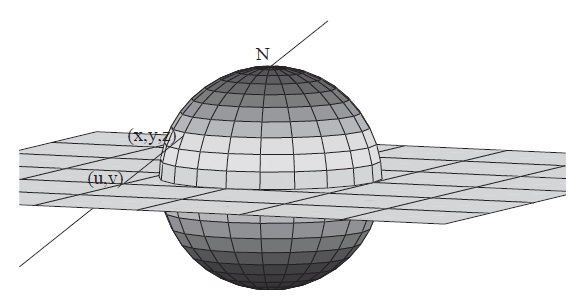
\includegraphics[scale=0.5]{proyeccionestereografica.png}
\caption{Proyección estereográfica que usamos para definir el infinito.}
\end{figure}
 
Decimos que una región $R$ contiene a $z = \infty$ si tiene una intersección no nula con todos los $\varepsilon$-entornos, es decir, si no está acotada. Definiendo estos entornos como:

\begin{equation}
\varepsilon - \mathrm{entorno:} \ \ \{ |z|>1/\varepsilon, \varepsilon>0 \}
\end{equation}


Si $f(z)$ es analítica en $z=\infty$ entonces $f(1/w)$ es analítica en $w=0$. En caso contrario se dice que $f(z)$ es \textbf{singular en el infinito}. \\

Además si $f(z)$ es analítica en $R / |z| > r / r \in \mathbb{R}$, y $f(1/w)$ es \textit{singular} en $w=0$ decimos que $f(z)$ posee una \textbf{singularidad aislada en el infinito}. Sera un  \textit{polo, singularidad evitable o esencial} en función de si $f(1/w)$ tiene un \textit{polo, singularidad evitable o esencial} en $w=0$. \\

\subsection{Residuo en el infinito}

Si hay una singular aislada en $w=0$ para $f(1/w)$ teneos que podemos desarrollar la serie de Laurent para un disco alrededor de este punto de tal forma que:

$$f(1/w) = \sum_{n= -\infty }^{\infty} c_n w^n \Longrightarrow f(z) = \sum_{n= -\infty }^{\infty} c_n z^{-1}$$

por lo que el residuo de $f(z)$ en $\infty$ se puede definir como:

\begin{equation}
\Res  (f(z), \infty) = - c_1
\end{equation}

donde $c_1$ será el primer término de la serie de Taylor de $f(1/w)$ centrado en $a=0$. Ahora entenderemos porque lleva el símbolo negativo. Si no hay ninguna singularidad aislada en $w=0$ desarrollamos el siguiente teorema:

\begin{theorem}
sea $C$ una curva de Jordan orientada en el sentido contrario al de las agujas del reloj, y supongamos que $f(1/w)$ no tiene una singularidad en $w=0$. Si $f(z)$ es analítica sobre la curva $C$ y en el exterior excepto en un número finito de singularidades aisladas (suponemos que no hay en el interior), tenemos que

$$ \oint_C f(z) \D z = 2 \pi i \sum_{j=0}^N \Res (f(z),a_j) $$

donde $a_0 = \infty$.
\end{theorem}

\begin{corollary}
si  $f$ es analítica en $\bar{\mathbb{C}}$ excepto en un número finito de singularidades aisladas en $|z| \leq  \infty$ entonces:

$$ \sum_{k=0}^N \Res  (f,a_k) = 0 $$

lo cual se deduce del teorema anterior ya que $I=2 \pi i\sum_{i=1}^{\infty} \Res (f,a_i) = - 2 \pi i \Res(f,a_0)$. 

\end{corollary}




\shadowbox{\textbf{Ejemplo 5.3}}

\hrulefill


Calcular el polo $z=\infty$ conociendo los polos simples en $z=0$ y $z=1$ de la función:

$$ f(z) = \frac{5 z}{z-1} $$

Está claro que los residuos simples son:

$$ \Res(f,0) = 2 \quad \quad \quad \Res(f,1) = 3 $$

Por lo que $\Res(z=\infty)  = 5$. Veámoslo:

$$ \Res (f,z=\infty) = - \Res(\dfrac{1}{w^2} f(1/w),0) $$


donde claramente:

$$ \dfrac{1}{w^2} f(w) =  \dfrac{1}{w} \dfrac{5-2w}{1-w} =F(w) \Longrightarrow  \Res(F(w),0) = 5 $$


\hrulefill \\




\newpage
\chapter{Trasformadas Integrales}
\section{Trasformadas integrales general}

Sea $f(x)$ función de variable real, y sea $N(k,x)$ (no necesariamente real) una función de dos variables reales ($k$ y $x$ son reales). Definimos como \textbf{trasformada integral} de $f$ con \textbf{núcleo} $N(x,k)$ a:

\begin{equation}
\widehat{f}(k) = \int_{-\infty}^{\infty} N(k,x) f(x) = N(f(x),k)
\end{equation}

también expresada como:

\begin{equation}
\hatf (k) = N(f(x),k)
\end{equation}


Las dos trasformadas integrales mas famosas son:


\begin{itemize}
\item \textbf{Trasformada de Fourier:} es una trasformada cuyo núcleo es:

\begin{equation}
N(k,x) = F(k,x) = \dfrac{1}{\sqrt{2 \pi}} e^{ikx}
\end{equation}

\item \textbf{Trasformada de Laplace:} es una trasformada cuyo núcleo es:

\begin{equation}
N(k,x) = L(k,x) =  \left\lbrace \begin{array}{ll} 0 & x < 0 \\ e^{-kx} & x \geq 0 \end{array} \right.
\end{equation}
\end{itemize}

Las trasformadas integrales tienen una serie de propiedades comunes, ya que todas ellas tienen una definición común. De hecho la mayoría de las propiedades para cada trasformada que vamos a ver tienen mucha relación entre sí, ya que entre ellas solo cambia el núcleo o los límites de integración. Una de las propiedades mas relevantes es que las trasformadas son lineales, lo cual es trivial ya que la suma de las integrales es la integral de la suma:

\begin{equation}
N(a f(x) + b g(x),k) = a N(f(x),k) + b N(g(x),k)
\end{equation}


\subsection{Funciones definidas a trozos y aboslutamente integrables}

Definimos como \textbf{función absolutamente integrable} en un intervalo $I=[a,b]$ a aquella función tal que:

\begin{equation}
\int_I |f(x)| < \infty
\end{equation}

Decimos que $f(x)$ es una \textbf{función continua a trozos} en el intervalo [$a,b$] si la función es tal que en dicho intervalo podemos encontrar un número finito de trozos [$a,a_1$],...[$a_N,b$] donde $f(x)$ es continua, además que:


$$ \lim_{x \rightarrow a_i^+} f(x) = A, \lim_{x \rightarrow a_i^-} f(x) = B \Longrightarrow A,B \in \mathbb{R}   $$

pero $A$ y $B$ no son necesariamente iguales. Es decir, existen los límites por ambos lados, pudiendo haber discontinuidades de salto. Toda función continua es una función continua a trozos (un único trozo).

\section{Trasformadas de Fourier}

La \textbf{trasformada de Fourier} esta definida como:

\begin{equation}
F(f(x),k) = \hatf(k) = \dfrac{1}{\sqrt{2 \pi}} \inti e^{ikx} f(x) \D x
\end{equation}

La única condición que impone la trasformada de Fourier es que la función $f(x)$ sea \textit{absolutamente integrable}. \\

Al igual que existe una trasformada de Fourier existe una \textbf{trasformada inversa de Fourier}, que nos devuelve la función $f(x)$ a partir de la trasformada $\hatf(k)$. Esta es:

\begin{equation}
f(x) = \dfrac{1}{\sqrt{2 \pi}} \inti e^{-ikx} \hatf (k) \D k = F^{-1}[\hatf (k),x]
\end{equation}

A grandes rasgos, trasformada de Fourier lo que hace es transformar una función (señal) en función del tiempo a una en función de la frecuencia (k = frecuencia angular, w). Al igual que la serie de Fourier descompone una función periódica en función de sus componentes armónicas, la trasformada de Fouerier genera una función (señal) continua función de la frecuencia.\\


\shadowbox{\textbf{Ejemplos}} 

\hrulefill \\


Calcula la transformada de Fourier de $f(x)$ tal que

$$ f(x) = \left\lbrace \begin{array}{ll}
1 & |x|<a \\
0 & |x|>a 
\end{array} \right. $$

Tenemos que:

$$ F(x) = \dfrac{1}{\sqrt{2 \pi}} \inti f(x) e^{ikx} \D x =  \dfrac{1}{\sqrt{2 \pi}} \int_{-a}^a  e^{ikx} \D x =   \dfrac{1}{\sqrt{2 \pi}} \left[ \dfrac{1}{ik} e^{ikx} \right]_{-a}^a = \dfrac{2}{\sqrt{\pi}}  \dfrac{\sin (ka)}{k}  $$

donde hemos usado que $e^{ika}-e^{-ika} = 2 \sin(ka)$. En la figura \ref{Fig:6.2-1} podemos ver las funciones.

\hrulefill \\

\hrulefill \\


Calcula la transformada de Fourier de $f(x)$ tal que

$$ f(x) = e^{-ax^2}$$

Tenemos que:

$$ F(k) = \dfrac{1}{\sqrt{2 \pi}} \inti e^{-ax^2} e^{ikx} \D x =  \dfrac{1}{\sqrt{2 \pi}} \inti e^{-a(x-ik/a2)^2 - k^2/a4} \D x =  \dfrac{e^{-k^2/a4}}{\sqrt{2 \pi}} \inti e^{-a(x-ik/a2)^2} \D x $$

si hacemos el cambio de variable de integración $y = (x-ik/2)$ tal que $\D y = \D x$, podemos deducir que:

$$ F(k) = \dfrac{e^{-k^2/a4}}{\sqrt{2 \pi}} \inti e^{-a y^2} \D y = \dfrac{1}{\sqrt{2 a}} e^{-k^2/a4} $$

ya que la integral:

$$ \inti e^{ay^2} \D y =  \sqrt{\dfrac{\pi}{a}}  $$

\hrulefill

\begin{figure}[h!] \centering
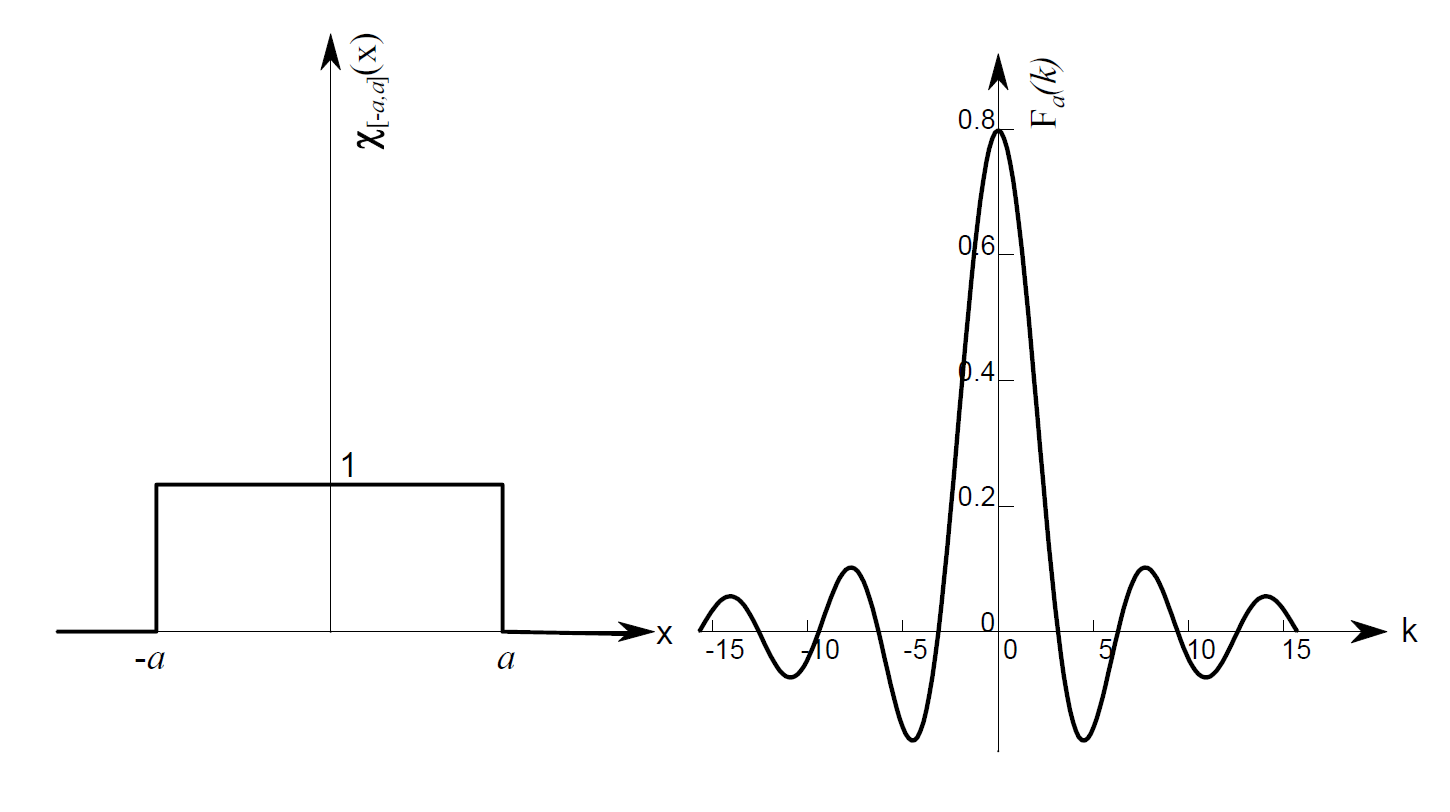
\includegraphics[scale=0.5]{trasformadafourier1.png}
\caption{representación gráfica de una función $f(x)$ cuadrada y su trasformada de Fourier}
\label{Fig:6.2-1}
\end{figure}


\subsection{Trasformadas para funciones pares e impares} 

Las trasformadas de fourier se pueden relacionar con las trasformadas del seno y del coseno, usando la expresión trigonométrica de la exponencial compleja. Sea $f^+(x)$ una función par y otra $f^-(x)$ impar. Entonces tenemos que:

\begin{equation}
f^+ = \left\lbrace \begin{array}{ll} f(-x) & x < 0 \\ f(x) & x \geq 0 \end{array} \right. \tquad f^- = \left\lbrace \begin{array}{ll} -f(-x) & x < 0 \\ f(x) & x \geq 0 \end{array} \right.
\end{equation}


Es fácil de ver que para una función par/impar tenemos que la trasformada integral de Fourier será:

\begin{equation}
\hatf^{\pm} (k) = \inti \dfrac{1}{\sqrt{2 \pi}} e^{ikx} f^{\pm} (x) \D x = \dfrac{1}{\sqrt{2 \pi}} \ccorchetes{\pm \int_{0}^\infty e^{ikx} f(x) \D x + \int_{0}^\infty e^{ikx} f (x) \D x }
 \end{equation}
 
O sea para cada cada función:
 
\begin{equation}
\hatf^{+} (k) = \dfrac{1}{2 \pi} \int_0^\infty f(x) (e^{ikx} + e^{-ikx} ) \D x = \sqrt{ \dfrac{2}{\pi} } \int_0^\infty f(x) \cos(kx) \D x
\end{equation}
\begin{equation}
\hatf^{-} (k) = \dfrac{1}{2 \pi} \int_0^\infty f(x) (e^{ikx} - e^{-ikx} ) \D x = i \sqrt{ \dfrac{2}{\pi} }  \int_0^\infty f(x) \sin(kx) \D x
\end{equation}

Que son las \textbf{trasformadas del coseno} y \textbf{del seno} respectivamente. Es decir, la trasformada de Fourier se transforma en estas dos dependiendo de si la función es par o impar.\\


\subsection{Teorema integral de Fouerier}

\begin{theorem}
sean $f(x)$ y $f'(x)$ funciones continuas a trozos y absolutamente integrable, para todo $x \in  \mathbb{R}$ tenemos que la integral de Fourier converge a $\frac{1}{2} \left[ f(x+0) + f(x-0) \right]$, o en otras palabras:

$$  \dfrac{1}{2} \left[ f(x+0) + f(x-0) \right] = \dfrac{1}{\pi} \into \D k \into \D t f(t) \cos [k(t-x)]   $$

si $f(x)$ es continuo en $x$ tenemos que $f(x+0) = f(x-0) = f(x)$. 

\end{theorem}

\subsection{Lema de Riemann-Lebesque}

\begin{lemma}[Lema de Riemann-Lebesque]
sea $f(x)$ una función continua a trozos y absolutamente integrable en el intervalo [$a, \infty$), se verificará que:

$$ \lim_{k \rightarrow \infty} \int_a^\infty f(x)  \sin (k x) \D x  = \lim_{k \rightarrow \infty} \int_a^\infty f(x)  \cos (k x) \D x = 0$$
\end{lemma}

Lo cual implica que la trasformada de Fourier cuando $k$ tiende a infinito esta es cero:

\begin{equation}
 \lim_{k \rightarrow \infty} \hatf (k) = 0 
\end{equation}

\subsection{Lema de localización}

\begin{lemma}
sean $f(x), f'(x)$ continua a trozos en $[0,a]$ tal que $0<a<\infty$, se verificará que:
$$ \lim_{\lambda  \rightarrow \infty} \int_ 0^a \D x f(x) \dfrac{\sin (\lambda x)}{x} = \dfrac{\pi}{2} f(0+) $$
\end{lemma}


\subsection{Propiedades de la Trasforamda de Fourier}

Para la trasformada de Fourier tenemos las siguientes propiedades:

\begin{enumerate}

\item \textit{Reescalado}:

$$ F(f(ax),k) = \dfrac{1}{|a|} F(f(x),k/a) $$

\item \textit{Retardo}:

$$ F(f(x-a),k) = e^{ika} F(f(x),k) $$

\item \textit{Traslado}:

$$ F(e^{ixa} f(x),k) = F(f(x),k+a) $$

\item \textit{Conjugado}:

$$ F(f^* (\pm x), k) = F(f(x), \pm k)^* $$

\item \textit{Derivada de la función}:

$$ F(f'(x),k) = - ik F(f(x),k)  \Longrightarrow F(f`'^{n},k) = (-ik)^n F(f(x),k) $$

\item \textit{Derivada de la trasformada}:

$$ F(x f(x), k) = -i \hatf'(k) \Longrightarrow F(x^n f(x), k) = (-i)^n \dfrac{\D^n}{\D k^n} \hatf (k) $$

\item \textit{Composición}:

$$ \inti F(k) g(k) e^{ikx} \D k = \inti f(t) G(t-x) \D t \tquad G(t) = F(g(x),t) $$

\end{enumerate}

Existe un teorema que nos dice cuando es la trasformada continua y acotada:

\begin{theorem}
si $f(x)$ es una función continua a trozos y absolutamente integrable tenemos entonces que la trasformada de Fourier $\hatf (k)$ es continua y acotada de $-\infty$ a $\infty$.
\end{theorem}

\subsection{Convolución de Fourier}


\begin{definicion}
sean dos funciones integrables $f(x)$ y $g(x)$, denotamos por $(f * g)(x)$ a la \textbf{convolución}, que se define como:

\begin{equation}
(f * g)(x) = \dfrac{1}{\sqrt{2 \pi}} \int_{-\infty}^{\infty}  f(x-t) g(t) \D t
\end{equation}

siendo el factor $1/\sqrt{2 \pi}$ un factor que no afecta a al definición de la convolución.
\end{definicion}


Con esta definción queda claro que tiene las siguientes propiedades:

\begin{enumerate}
\item \textit{Comutativa}: $$ f * g = g * f $$
\item \textit{Asociativa}: $$ f * (g * h) = (f * g) * h $$
\item \textit{Distributiva}: $$ (a f + b g) * h = a (f * h) + b (g * h) $$
\end{enumerate}

La razón por la que definimos la convolución se expresa en el siguiente teorema, que será de gran utilidad tanto para la resolución de funciones integrales y diferenciales:

\begin{theorem}[teorema de la convolución]
si $F(f(x),k) = F(k)$ y $F(g(x),k) = G(k)$ entonces tenemos que:

$$ F(f(x) * g(x) , k) = F(x) G(x) $$
\end{theorem}

es decir el teorema de la convolución relaciona la trasformada de la convolución con el producto de las trasformadas. 


\begin{theorem}[teorema de Parseval] si $F(f(x),k)  = F(k)$ y $F(g(x),k) = G(x)$ tenemos que:

$$  \inti f(x) \overline{g(x)} \D x   = \inti F(k) \overline{G(k)} \D k  $$
\end{theorem}

y si definimos como $| f(x)| ^2 = f(x) \overline{f(x)}$ obtenemos que:

\begin{equation}
\inti \D x |f(x)|^2 = \inti \D k |\widehat{f}(k)|^2 
\end{equation}


\subsection{Desigualdades}

\begin{equation}
(\Delta x)^2(\Delta k)^2 = \dfrac{\inti \D x x^2 |f(x)|^2 \inti \D k (k - \bar{k})^2 |\hatf(k)|^2}{\inti \D x |f(x)|^2 \inti \D k |f(k)|^2}
\end{equation}


\begin{theorem}[desigualdad de Cauchy-Schwartz]
este teorema nos dice que:

$$ \parentesis{\inti \D x |f(x)|^2} \parentesis{\inti \D x |g(x)|^2} \geq \left| \inti \D x f(x) g^* (x) \right|^2   $$
\end{theorem}

\begin{theorem}
si $|xf(x)|^2$ es absolutamente integrable:
$$ \Delta x \Delta k \geq \frac{1}{2} $$
\end{theorem}



\section{Trasformada de Laplace}

La trasformada de Laplace está definida como:

\begin{equation}
L(f(t),p) = \tf (p) = \int_0^\infty e^{-pt} f(t) \D t
\end{equation}

donde se tiene que verificar que $\Real (p) > 0$. La función inversa de la trasformada de Laplace viene dada por:

\begin{equation}
L^{-1} (\tf(p),t) = f(x) = \dfrac{1}{2 \pi i} \int_{c- i \infty}^{c+i\infty} e^{pt} \tf (p) \D p \tquad c > 0 
\end{equation} \\


\begin{flushleft}
\shadowbox{\textbf{Ejemplo}} 

\hrulefill \\

Calcula la transformada de Laplace de $f(x)$ tal que

$$ f(x) = e^{ax}   $$

Se tiene que verificar $\Real(p)>a$ (véase \ref{Subsec:6.3.3}). La solución será:

$$ F(x) =  \into f(t) e^{-pt} \D t = \into e^{-(p-a)t} = \dfrac{1}{p-a}  $$
\hrulefill \\


\end{flushleft}

Una vez hemos calculado la integral para la exponencial normal las funciones que se pueden escribir como suma de exponenciales (por ejemplo las trigonométricas en función de exponenciales complejas o las hiperbólicas) son triviales. A continuación realizaremos el estudio para dos de ellos (uno para el coseno otro para el seno hiperbólico). Los otros se harán de manera completamente análoga. \\



\begin{flushleft}
\shadowbox{\textbf{Ejemplos}} 

\hrulefill \\
Calcula la trasformada de Laplace de $f(t)$ tal que:

$$ f(t) = \cos at \tquad \Real(p) > a $$

Tenemos que el coseno se puede escribir en función de exponenciales complejas:

$$ L(p) = \into \parentesis{\dfrac{e^{iat}+e^{-iat}}{2}} e^{-pt} \D t = \dfrac{1}{2} \left[ \into e^{iat} e^{-pt} \D t + \into e^{-iat} e^{-pt} \D t \right] = \dfrac{1}{2} \left[ \dfrac{1}{p-ia} + \dfrac{1}{p+ia} \right] $$

Ahora si despejamos podemos obtener que:

$$ L(p) = \dfrac{1}{2} \left[ \dfrac{p+ia}{p^2+a^2} + \dfrac{p-ia}{p^2+a^2} \right] = \dfrac{p}{p^2 + a^2}  $$

\hrulefill \\

\hrulefill \\
Calcula la trasformada de Laplace de $f(t)$ tal que:

$$ f(t) = \sinh at $$

Tenemos que el coseno se puede escribir en función de exponenciales complejas:

$$ L(p) = \into \parentesis{\dfrac{e^{at}-e^{at}}{2}} e^{-pt} \D t = \dfrac{1}{2} \left[ \into e^{at} e^{-pt} \D t - \into e^{-at} e^{-pt} \D t \right] = \dfrac{1}{2} \left[ \dfrac{1}{p-a} - \dfrac{1}{p+a} \right] $$

Ahora si despejamos podemos obtener que:

$$ L(p) = \dfrac{1}{2} \left[ \dfrac{p+a}{p^2+a^2} - \dfrac{p - a}{p^2 - a^2} \right] = \dfrac{a}{p^2 - a^2}  $$

\hrulefill \\ 
\end{flushleft}


De hecho se puede obtener el seno y el coseno a partir de los senos y cosenos hiperbólicos. De manera general obtenemos que:

\begin{equation}
L (\sin at,p) = \dfrac{a}{p^2 + a^2} \tquad 
L (\cos at,p) = \dfrac{p}{p^2 + a^2}
\end{equation}
\begin{equation}
L (\sinh at,p) = \dfrac{a}{p^2 - a^2} \tquad 
L (\cosh at,p) = \dfrac{p}{p^2 - a^2}
\end{equation}



\subsection{Condiciones para la existencia de la trasformada de Laplace} \label{Subsec:6.3.3}

Una función $f(t)$ se dice que es una exponencial de orden $a$ si en el intervalo $0 \leq x \leq \infty$ existe una constante positiva $K$ tal que para todo $t >  T \ / \ T \in \mathbb{R}$ se verifica que:

\begin{equation}
|f(t)| \leq K e^{at}
\end{equation}

Esta condición se escribe en la mayoría de la bibliografía como:

$$ f(t) = O(e^{at}) \tquad cuando \ t \rightarrow \infty $$

Entonces la existencia de la trasformada de Laplace:

\begin{theorem}[existencia trasformada Laplace]
si una función $f(t)$ es continua a trozos en un intervalo infinito (0,T), y es $f(t)=O(e^{at})$, entonces la trasformada de Laplace \textbf{existe} para todo $p$ tal que $\Real( p ) > a$.\\
\end{theorem} 


\subsection{Trasformadas de Laplace para las derivadas}

El teorema que vamos a introducir es uno de los mas potentes e interesantes que podemos estudiar este tema. En líneas generales nos permite expresar la trasformada de Laplace de la n-ésima derivada en función de la trasformada de Laplace y algunas condiciones iniciales (ya veremos). \\

Esto es extremadamente útil a la hora de resolver ecuaciones diferenciales, ya que nos permitirá pasar de una ecuación diferencial expresada en función de $f(x)$ a una de orden menor en función de $\tilde{f}(p)$ fácilmente resoluble. Luego aplicando la trasformada inversa de Laplace obtendremos $f(x)$. Ya veremos algún ejemplo, ahora introduzcamos el teorema en cuestión:

\begin{theorem}
Si $L(f(t),p) = \tilde{f}(p)$, entonces:
$$ \begin{array}{rll}  L(f'(t),p) & =  & p \tilde{f}(p)  - f(0) \\
L(f''(t),p) & = & p^2 \tilde{f}(p)-pf(0)-f'(0) \end{array} $$
o de manera general:

$$ L(f^{(n)} (t)) = p^n \tilde{f}(p) - p^{n-1} f(0) - p^{n-2} f'(0)- \cdots - pf^{(n-2)}(0) - f^{(n-1)}(0) $$\\
\end{theorem}


\subsection{Convolución de Laplace}

En primer lugar vamos a definir lo que es la convolución de Laplace, que en líneas generales será exactamente igual que la convolución de Fourier pero cambiando los límites de integración. 

\begin{definicion}
llamamos a $f(x)*g(x)$ \textbf{convolución} de $f(x)$ y $g(x)$ definida como:
$$ f(x)*g(x) = \int_0^x f(x- \tau) g(\tau) \D \tau $$
\end{definicion}

con las mismas propiedades que la de Fourier:

\begin{enumerate}
\item \textit{Comutativa}: $$ f * g = g * f $$
\item \textit{Asociativa}: $$ f * (g * h) = (f * g) * h $$
\item \textit{Distributiva}: $$ (a f + b g) * h = a (f * h) + b (g * h) $$
\end{enumerate}


Ahora introducimos el siguiente teorema que relaciona la convolución con el producto de trasformadas:

\begin{theorem}[teorema de la convolución]
si $L(f(x),p) = \tilde{f}(p)$ y $L(g(x),p) = \tilde{g}(p)$ entones se verificará que:
$$ L(f(x) * g(x),p) = L(f(x),p) L(g(x),p) = \tilde{f}(p) \tilde{g}(p) $$
\end{theorem}

\subsection{Propiedades de la Trasformada de Laplace}

Tenemos varias propiedades muchas de ellas análogas a la trasformada de Fourier:

\begin{enumerate}

\item \textit{Reescalado}:

$$ L(f(at),p) = \dfrac{1}{|a|} L(t,p/a) $$

\item \textit{Retardo}:

$$ L(f(t-a),p) = e^{-pa} L(f(t),p) $$

\item \textit{Traslado}:

$$ L(e^{-ax} f(t),k) = L(t,p+a) $$

\item \textit{Derivada de la trasformada}:

$$ L(t f(t), p) = - \tilde{f}'(p) \Longrightarrow L(t^n f(t), p) = (-1)^n \dfrac{\D^n}{\D p^n} \tilde{f} (p) $$

\end{enumerate}

Veamos ahora algunos ejemplos de como aplicar estas propiedades a la resolución de transformadas de Laplace:

\begin{flushleft}
\shadowbox{\textbf{Ejemplos}} 

\hrulefill \\

Estas propiedades se pueden usar para obtener algunas de las trasformadas mas relevantes. Sabemos que la trasformada de $f(t) = 1$ es $\tf = 1/p$. Veamos como resolver ahora $g(t) = t^n$, tal que $g(t)=t^n f(t)$. Supongamos en primer lugar que $n \in \mathbb{N}$. Tenemos entonces que:

$$ L(g(t),p) = \into t^n e^{-pt} \D t $$

podemos hacerlo de dos maneras: hacer n integrales por partes, o usar la cuarta propiedad, lo cual es muchísimo mas rápido y sencillo. Sabemos que:

$$ L(t^n f(t), p) = (-1)^n \dfrac{\D^n}{\D p^n} \tilde{f} (p) $$

si $f(t)=1$, $\tf = 1/p$ y las $n$-ésimas derivadas vienen dadas por:

$$ L(g(t),p) = (-1)^n \left( (-1)^n \dfrac{n!}{p^{(n+1)}} \right) = \dfrac{n!}{p^{(n+1)}}$$

\hrulefill \\

\hrulefill

Ahora supongamos que $a \notin \mathbb{N}$ y es un número real cualquiera tal que $a > -1$. Sea $g(t)$ tal que:

$$ g(t) = t^a $$

Entones tendremos que:

$$L(g(t),p) = \into t^a e^{-pt} \D t $$

Usamos el cambio $pt = x$ de tal manera que:

$$ L(g(t),p) = \dfrac{1}{p^{a+1}} \into x^a e^{-x} \D x = \dfrac{\Gamma(a+1)}{p^a} $$

Siendo $\Gamma (a+1)$ la \textbf{función gamma} definida como:

\begin{equation}
\Gamma (a+1) = \into x^a e^{-x} \D x
\end{equation}

Tal que si $a \in \mathbb{N}$ tenemos que $\Gamma (a+1) = a!$

\hrulefill 

\end{flushleft}

\begin{figure}[h!] \centering
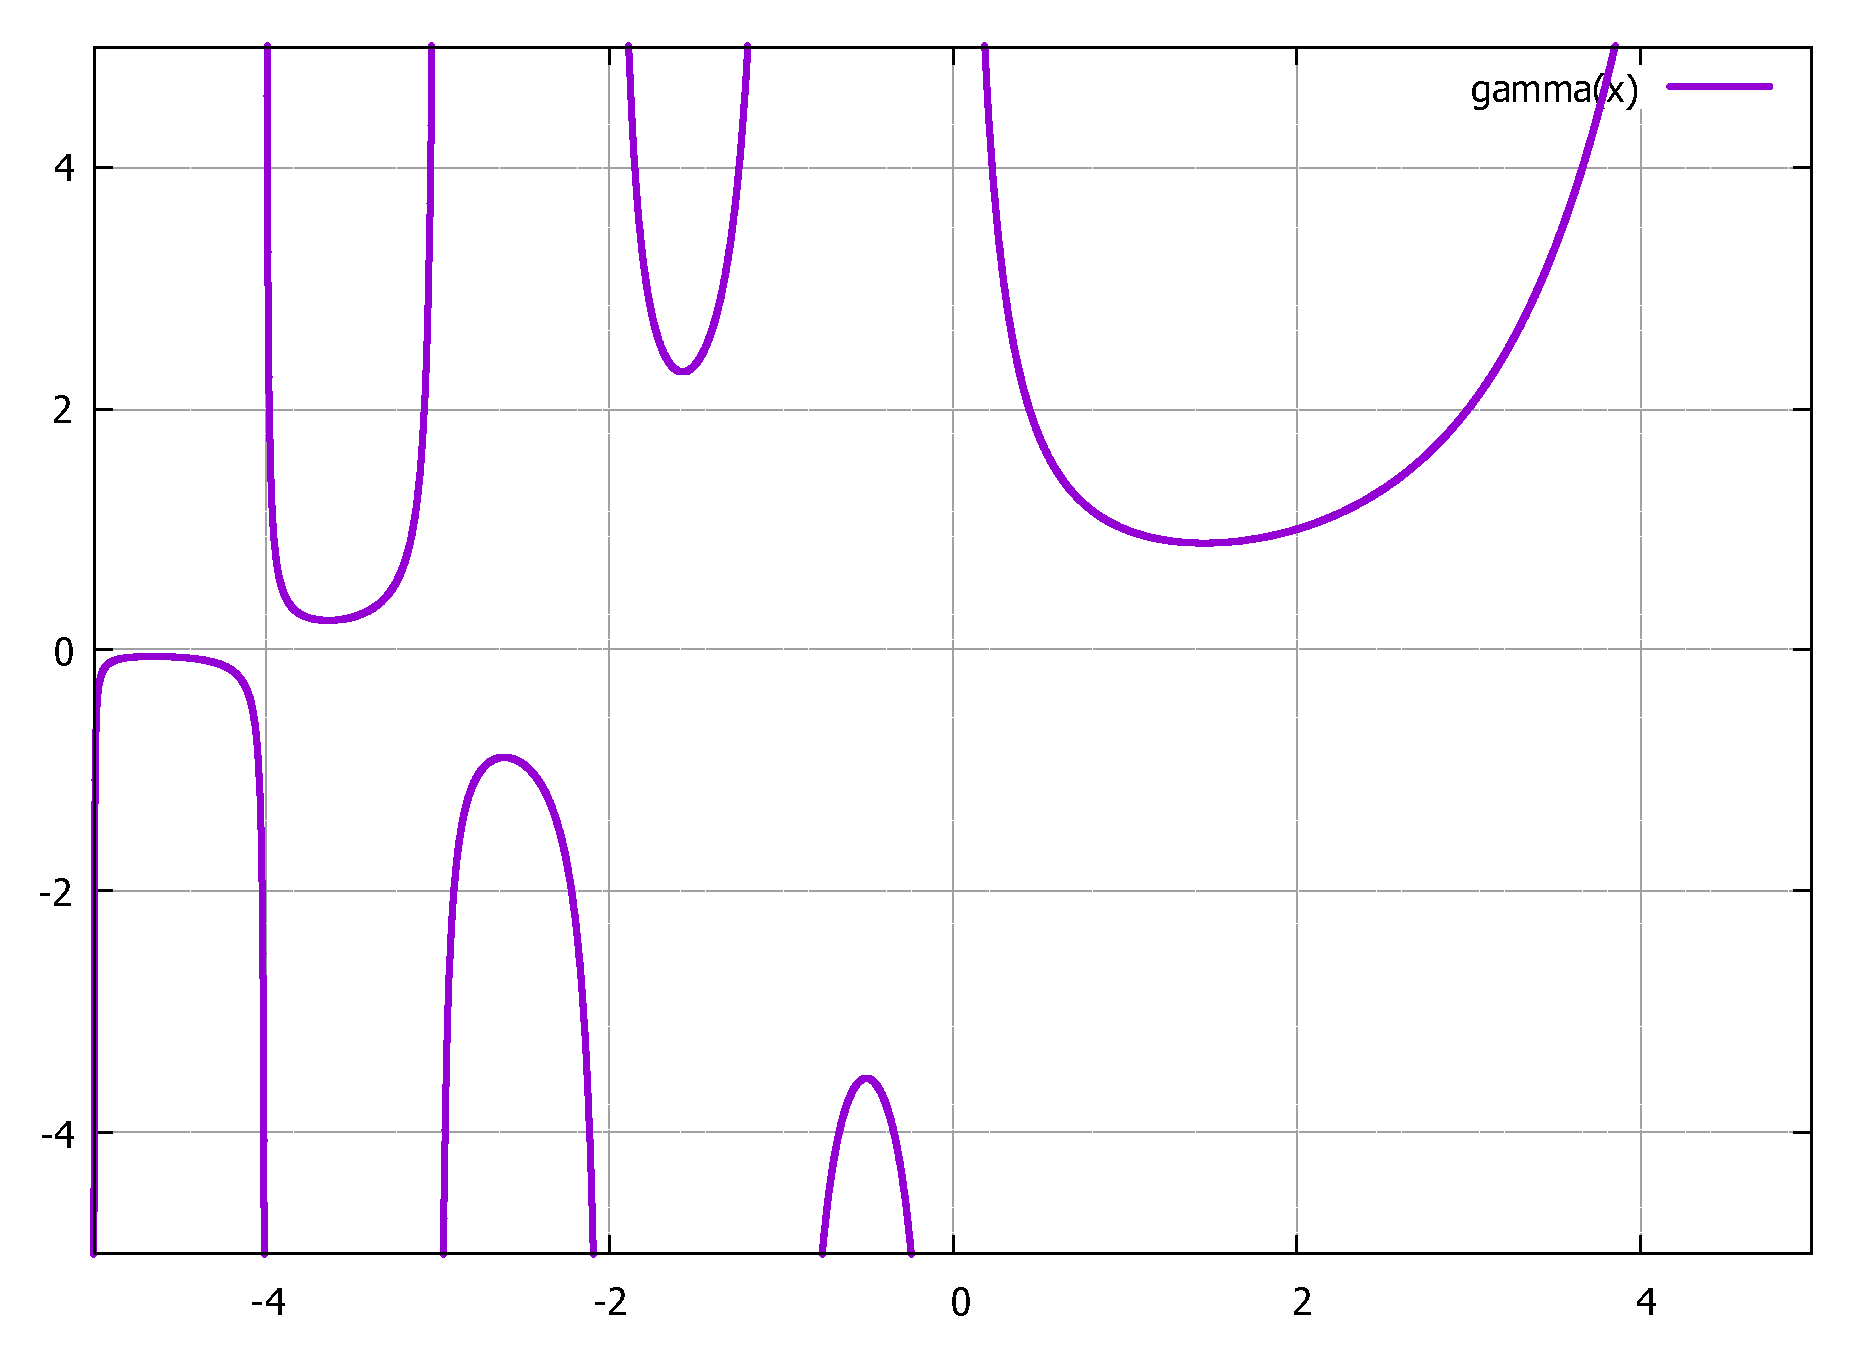
\includegraphics[scale=0.5]{gammafunction.pdf}
\caption{función gamma}
\end{figure}

\newpage


\chapter{Funciones generalizadas}


\section{Introducción}

Las funciones generalizadas surgen para dar un marco matemático y riguroso a ciertas idealizaciones empleadas el problemas físicos. Por ejemplo la carga puntual localizada en el origen de coordenadas debería ser representada por una función que solo es distinta de cero en el origen, limitándonos a un espacio unidimensional ($x \in \mathbb{R}$), y designando a la distribución de carga puntual por $\delta (x)$. Esta debe verificar que:

\begin{equation}
\inti \delta (x) \D x = 1
\end{equation}

A esta función la llamaremos \textbf{delta de Dirac}. Además debe verificar que $\delta (x) = 0 \ \forall x \neq 0$. Para que se cumpla la integral $\delta (x)$ debería poder definirse como:

\begin{equation}
\delta (x) = \left\lbrace \begin{array}{ll}
0 & x \neq 0 \\
\infty & x = 0
\end{array}
\right.
\end{equation}

Pero no existe ninguna función ordinaria que verifique esto. Una forma de definirla sería como el límite de alguna  sucesión de funciones $\{ \delta_n (x) \}$ tal que su integral en todo el espacio sea 1, y que tuviera un máximo en $x=0$ cada vez más pronunciado $n \rightarrow \infty$. Una de estas podría ser:

$$  \delta_n (x) = \sqrt{\dfrac{n}{\pi}} e^{-nx^2} $$

de tal forma que la delta de Dirac:

$$ \delta (x) = \lim_{n \rightarrow \infty} \{  \delta_n (x)  \}  $$

\begin{figure}[h!] \centering
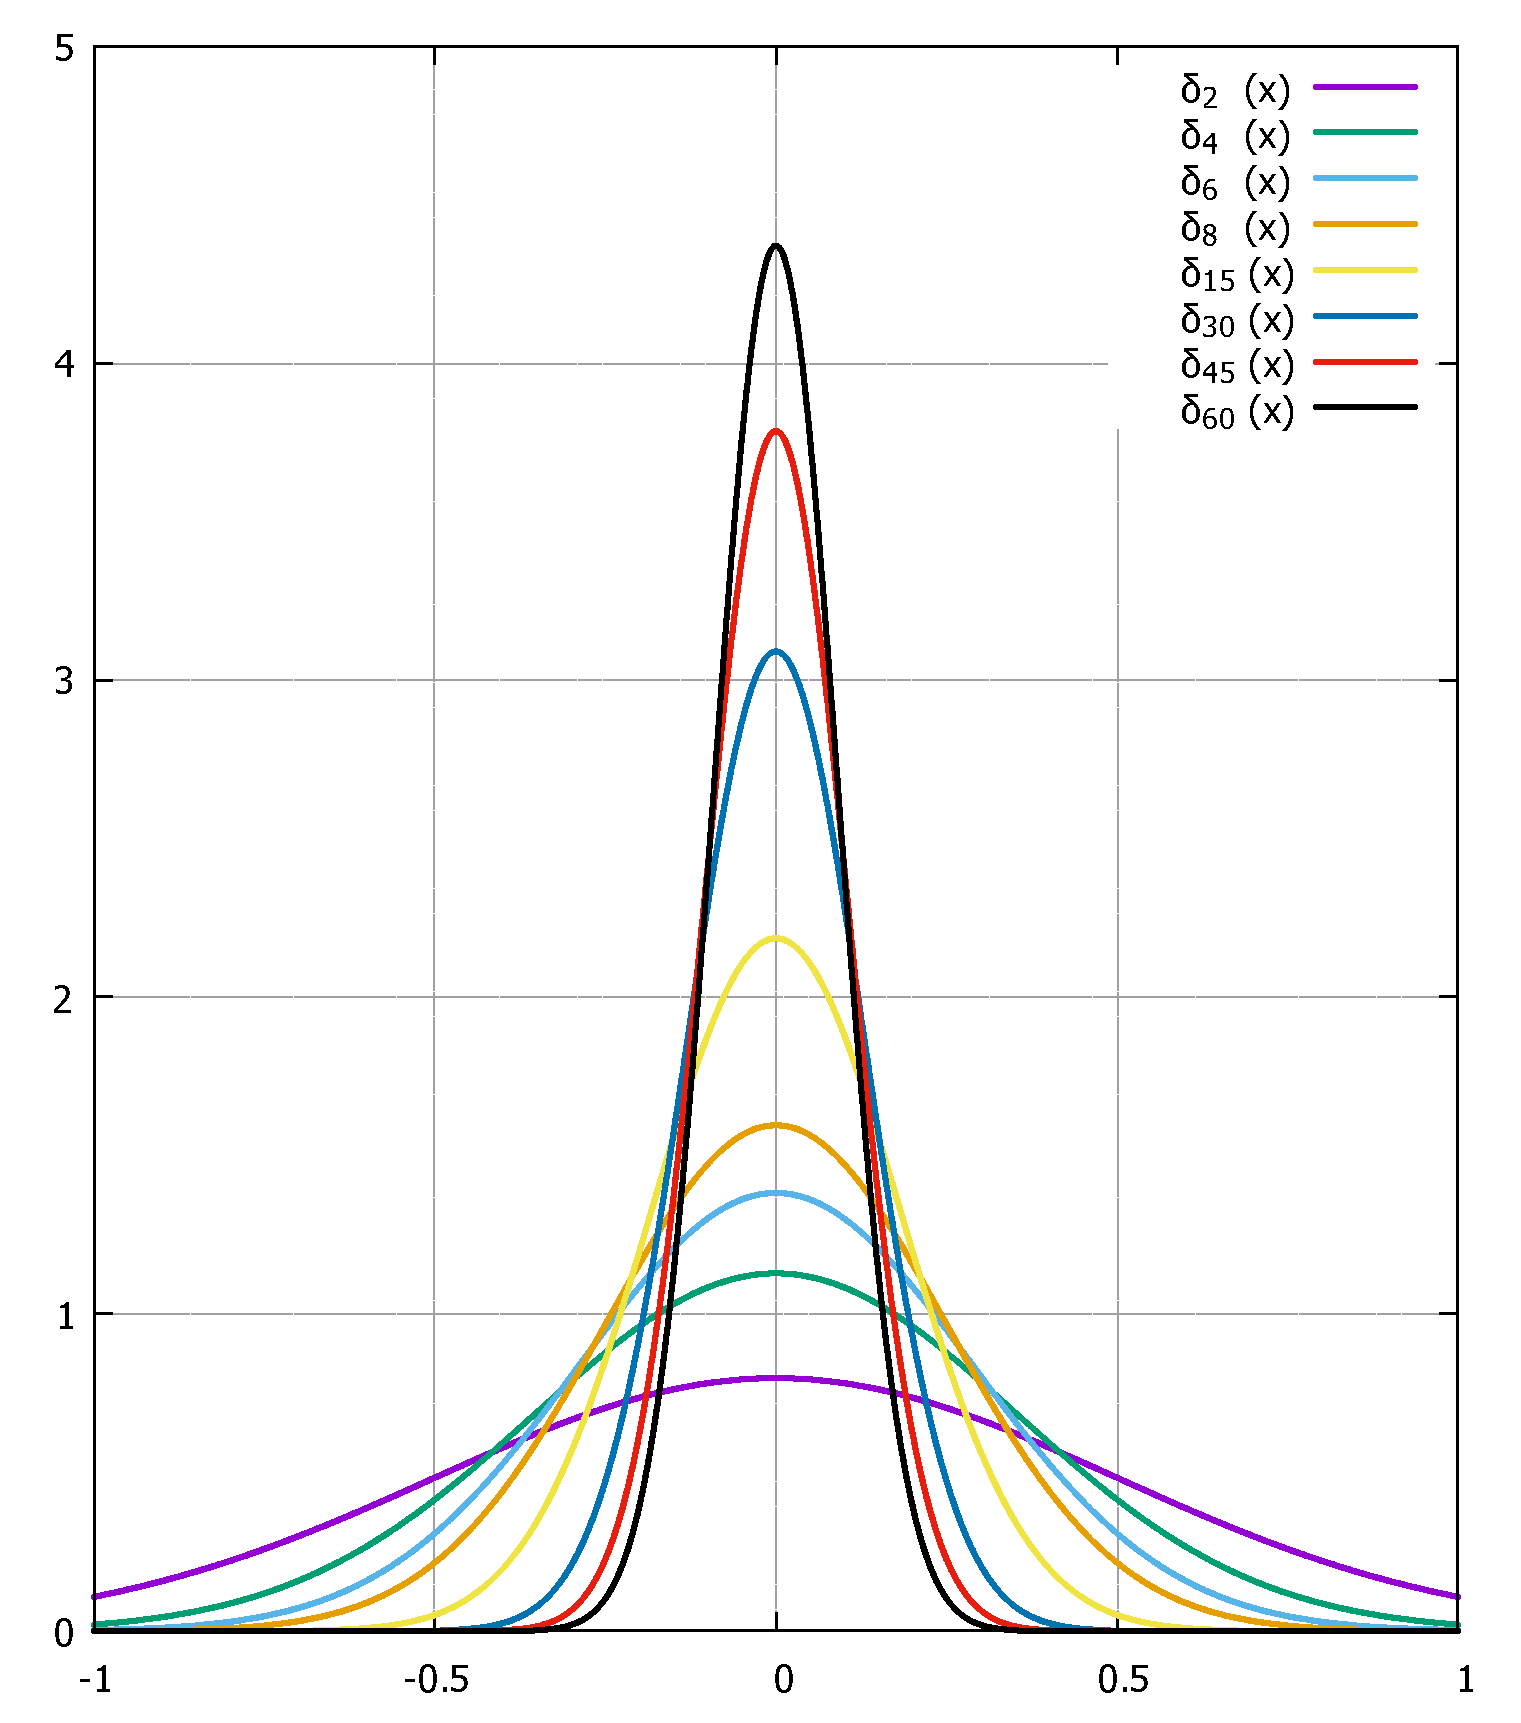
\includegraphics[scale=0.5]{deltadirac.pdf}
\caption{delta de dirac a medida que $n$ crece}
\end{figure}

Así es como se define una función en el sentido no ordinario. Básicamente es definir a las funciones no ordinarias como el límite de funciones ordinarias. Esto es análogo al proceso de obtener números reales como el límite de sucesiones de Cauchy de números racionales, tal y como:

$$ e = \lim_{n \rightarrow \infty} \parentesis{1+\dfrac{1}{n}}^n $$

\begin{definicion}
una función $f(x)$ definida en ($-\infty, \infty$) es de \textbf{decrecimineto rápido} si $\forall N \in \mathbb{N}$, $x^N f(x)$ está acotado cuando $x \rightarrow \infty $. Por ejemplo $e^{-x^2}$ es de decrecimiento rápido.
\end{definicion}

\begin{lemma}
Toda función de decrecimiento rápido está acotada para valores finitos de $x \in \mathbb{R}$, y es absolutamente integrable.
\end{lemma}

\begin{definicion}
una función $f(x)$ definida en ($-\infty, \infty$) es de \textbf{crecimiento lento} si $\forall N \in \mathbb{N}$, $f(x)/x^N $ está acotado cuando $x \rightarrow \infty $. Por ejemplo cualquier polinomio es de crecimiento lento.
\end{definicion}

\begin{lemma}
sean $f(x), g(x)$ de decrecimiento rápido y $h(x)$ de crecimiento lento. Entonces tenemos que $f \cdot h$ y $f + g$ son de decrecimiento rápido. 
\end{lemma}



\section{Clase Schwartz}



\begin{definicion}
$f(x) / x  \in \mathbb{R}$ pertenece a al \textbf{clase de Schwartz} $f (x) \in S$ si:
\begin{enumerate}
\item $f(x) \in C^{\infty}$
\item $f^{(p)}(x) = \dfrac{\D^p f(x)}{\D x^p}$ es de decrecemento rápido $\forall p \in \mathbb{N}$
\end{enumerate}
Un ejemplo es $e^{-x^2} \in S$.
\end{definicion}

\begin{lemma}
sea $f(x) \in S \ \exists \ n,p \in  \mathbb{N}$ implica que:
\begin{enumerate}
\item $f^{(n)} (x) \in S$
\item $x^p f(x) \in S$
\end{enumerate} 
\end{lemma}

Una consecuencia directa de que función sea de clase Schawrtz es que por ser de clase infinito que decrece rápidamente es que está acotada por lo que es absolutamente integrable y por lo tanto tiene trasformada de fourier. 

\begin{theorem}
si $f(x)$ es de clase Schwartz $f(x) \in S$, su trasformada de fourier es de clase Schwartz $\hatf (k) \in S$. 
\end{theorem}

\section{Sucesiones regulares y equivalentes}


\begin{definicion}
una sucesión $\{ f_n (x) \}$ de funciones de clase Schwartz ($f_n (x) \in S \ \forall n$) se dice \textbf{regular} si $\forall \varphi (x) \in S$ existe el límite:

$$ \lim_{n \rightarrow \infty} \int \D x f_n (x) \varphi (x)  $$
algunos ejemplos de sucesiones regulares son $f_n (x) = \sqrt{\pi/n} e^{-nx^2}$ o $f_n (x) = e^{-nx^2}$.
\end{definicion}

\begin{definicion}
dos sucesiones de funciones regulares $\{ f_n (x) \}  $ y $ \{ g_n(x) \}$ tal que $f_n, g_n \in S$ se dicen \textbf{equivalentes} si $\forall \varphi (x) \in S$ se verifica que:

$$ \lim_{n \rightarrow \infty} \int \D x f_n (x) \varphi (x) =  \lim_{n \rightarrow \infty} \int \D x g_n (x) \varphi (x)  $$

La expresión  $\{ f_n (x) \}  \sim \{ g_n(x) \}$ define las clases de equivalencia en el conjunto de las sucesiones regulares.
\end{definicion}
Algunos ejemplos de funciones equivalentes son:

\begin{itemize}
\item Son equivalentes $e^{-x^2/n^2}, e^{-x^2/n^4}$.

\item Son equivalentes $\sqrt{\frac{n}{\pi}} e^{-nx^2}, \sqrt{\frac{n \alpha}{\pi}} e^{-\alpha nx^2}, \frac{\beta n}{\sqrt{\pi}} e^{-\beta^2 n^2 x^2}$
\end{itemize}


\section{Funciones generalizadas}

\begin{definicion}
las clases de equivalencia de sucesiones regulares de funciones de clase Schwartz se denominan \textbf{funciones generalizadas}, y si $\{ f_n (x) \}$ es una de estas sucesiones, su clase de equivalencia se denotará a partir de ahora por:

$$ \left[ \{ f_n (x) \} \right] = f(x) $$
\end{definicion}

\begin{definicion}
si $f(x)$ es una función generalizada entonces $\forall \phi (x) \in S$ se denota como integral de la sucesión generalizada a:

$$ \inti \D x f(x) \varphi(x)  $$

que es equivalente a 

$$ \lim_{n \rightarrow \infty} \inti \D x f_n(x) \varphi (x) $$
\end{definicion}

Esta definición cobra sentido porque el límite de la integral $\lim_{n \rightarrow \infty} \int f_n \phi$ es el mismo para todas las sucesiones dentro de la clase de equivalencia. Podemos abusar del lenguaje y escribir que

\begin{equation}
\lim_{n \rightarrow \infty} f_n (x) = f(x)
\end{equation}
entendiendo que este límite solo será válido cuando $f_n (x),f(x)$ se multiplica por $\varphi (x) \in S$, y se integra entre $- \infty$ y $\infty$. Ahora vamos a definir las funciones generalizadas mas comunes, que son la función $1(0)$ y la función delta de Dirac $\delta(x)$. Veamos:

\begin{itemize}
\item Definimos la función generalizada (1) como 

$$ [ \{ e^{-x^2/n^2} \} ] \equiv (1) =  1 $$

tal que la integral siguiente:
 
$$ \lim_{n \rightarrow \infty} \inti e^{-x^2 / n^2} \varphi (x) \D x = \inti \D x \varphi (x) $$ 

\item Definimos la función generalizada \textbf{delta de Dirac} $\delta (x)$ como:

$$ [  \sqrt{\dfrac{n}{\pi}} \{ e^{-nx^2} \} ] \equiv \delta (x) $$

tal que la integral siguiente

$$ \lim_{n \rightarrow \infty} \inti \delta(x) \varphi (x) \D x = \varphi (0) $$ 
\end{itemize}

Es muy importante entender lo siguiente: en muchos ejercicios vamos a ver trasformadas de Fourier (o simplemente integrales) de funciones que no son absolutamente integrables, como puede ser un polinomio, pero que si son de clase Schwartz, y por lo tanto podemos definir una integral con funciones generalizadas. En ese caso asumiremos siempre que se harán integrales usando la función generalizada $1(0)$ implícita en ella (si usaramos la delta de dirac ya aparecería). 

\section{Operaciones entre funciones generalizadas}

Las operaciones entre funciones generalizadas deben verificar dos puntos: el primero es que la nueva sucesión tiene que seguir siendo compuesta por funciones de clase $S$, y el segundo punto es que diferentes elecciones de una misma clase de equivalencia dan lugar a sucesiones equivalentes al definir nuevas funciones generalizadas. Una propiedad interesante es la siguiente. Supongamos $f(x)$ función generalizada. Entonces si hacemos la integral de:

\begin{equation}
\inti \D x  f(ax+b) \varphi (x)  = \dfrac{1}{|a|} \inti \D x f(x) \varphi \parentesis{\frac{x-b}{a}} \D x
\end{equation}

que es trivial si hacemos el cambio $x' = ax+ b$. 

\subsection{Suma de funciones}

Sean $f(x)$ y $g(x)$ dos funciones generalizadas, definimos la suma $f(x) + g(x)$ como la nueva sucesión generalizada:

\begin{equation}
f(x) + g(x) = [ \{ f_n (x) + g_n (x) \} ]
\end{equation}
Para la suma se verifican estos puntos ya que para $\varphi \in S$ tenemos que

$$ \inti \D x [f(x) + g(x)] \varphi (x) = - \inti \D x f(x) \varphi (x) + \inti \D x g(x) \varphi (x) $$
y como son verificados por $f(x)$ y $g(x)$ por separado la suma los verificará. Esto implica que la función delta de dirac es par (a=-1, b=0). 

\subsection{Derivada de funciones}

Sean $f(x)$ una función generalizada, definimos la derivada $f ' (x)$ como la nueva sucesión generalizada:

\begin{equation}
f '(x) = [ \{ f_n ' (x) \} ]
\end{equation}
Además tenemos la siguiente relación (se deduce por partes):
\begin{equation} \inti \D x f '(x) \varphi (x) = \inti \D x f(x) \varphi '(x) 
\end{equation}
y como $f(x) \in S$, y por ser $\varphi (x) \in S, \varphi' (x) \in S$, tenemos que se verificarán ambos puntos. Veamos ejemplos de las derivadas de alguna de las funciones generalizadas que hemos visto.

\begin{itemize}
\item Sea la función generalizada (1) tenemos que:

$$ \inti \D x (1)' \D x = - \inti \D x \varphi'(x) = - [\varphi(\infty) - \varphi (-\infty)] = 0  $$

de lo que se puede deducir que:

\begin{equation}
(1)' = 0
\end{equation}

\item Sea la función generalizada $\delta (x)$, tenemos que:

$$ \inti \D x \delta ' (x) \varphi (x) = - \inti \D x \delta (x) \varphi ' (x) = - \varphi ' (0) $$

Por inducción se verificará que:

\begin{equation}
\inti \D x \delta^{(n)} \varphi (x) = (-1)^n \varphi^{(n)} (0)
\end{equation}

\end{itemize}

\begin{theorem}
si $f(x)$ es una función generalizada tal que $f'(x)= 0$ tenemos que $f(x)$ es una constante multiplicada por la función generalizada (1).
\end{theorem}

\subsection{Producto}

No existe una defunción satisfactoria del \textit{producto} de funciones generalizadas, ya que en general el producto de dos funciones de clase Schwartz no es de clase Schwartz. 

\begin{definicion}
una función ordinaria es de clase N ($f(x) \in N$) si.

\begin{enumerate}
\item $f(x)$ es infinitamente diferenciable en todo $\mathbb{R}$.
\item Todas las derivadas de $f(x)$ son de crecimiento lento 
\end{enumerate}

\end{definicion}

Entonces si $f \in N, g \in S$ se verificará que $f \cdot g \in S$ y por lo tanto si podamos definir un producto de funciones. Sea $\phi (x) \in N, f (x) \in S$, la sucesión $\{ \phi (x) f_n (x) \}$ es una sucesión regular de clase $S$. Aunque $\phi (x)$ no sea una función generaliza, el producto lo será. La integral se entonces:

\begin{equation}
\inti \D x (\phi (x) f(x)) \varphi (x) = \inti \D x f(x) (\phi (x) \varphi (x)) 
\end{equation}


\section{Transformadas de Fourier generalizadas}


\begin{definicion}
sea $f(x)$ una función generalizada definida por una sucesión regular. Entonces su transformada de fourier se defie como la clase de equivalencia de la sucesión regular $\{ \hatf_n (k) \}$ donde $\hatf_n (k) = F [f_n (x),k]$, tal y como la hemos definido para funciones ordinarias:

\begin{equation}
\hatf (k) = \dfrac{1}{\sqrt{2 \pi}} \inti  e^{ikx} f(x) \ \D x
\end{equation}
\end{definicion}

Las propiedades de la transformada de Fouerier de una función generalizada son exactamente análogas a las de una función ordinaria. Tenemos que:

\begin{itemize}
\item $ F(f(ax),k) = \frac{1}{|a|} F(f(x), k/a) $ \\

\item $ F(f(x-a),k) = e^{ika} F(f(x),k)$ \\

\item $ F(f^{(n)}(x),k ) = (-ik)^n F(f(x),k)$ \\

\item $ F(e^{iax} f(x),k) = F(f(x),k+a)$ \\

\item $ F( x^n f(x),k) = (-i)^n \hatf^{(n)} (k) $
\end{itemize}

También existe la inversa de la trasformada de Fourier tal que:

\begin{equation}
f_n (x) = F(\hatf (-k), x)
\end{equation}

por lo que podemos pasar de $\hatf(k)$ a $f(x)$ usando el operador $F$. \\

\shadowbox{\textbf{Ejemplo}} 

\hrulefill \\

Vamos a demostrar la siguiente relación:

\begin{equation}
F(1(0),k) = \sqrt{2 \pi} \ \delta (k)
\end{equation}

Tenemos que la transformada de fourier será:

$$ F(1(0),k) = \dfrac{1}{\sqrt{2 \pi}} \inti e^{ikx} e^{-x^2/n^2} \D x $$

Recordemos que esto ya lo hemos visto en el tema anterior de transformadas, que no es otro que la transformada de la función gaussiana. Entonces se verifica que:

$$ F(1(0),k) = \dfrac{1}{\sqrt{2 \pi}} \inti e^{-(x/n-ink/2)^2-n^2k^2/4} \D x = \dfrac{1}{\sqrt{2 \pi}} e^{-\frac{k^2 n^2}{4}} \inti e^{-(x/n-k n^2 / 4)} \D x = \dfrac{n}{\sqrt{2}} e^{-\frac{n^2 k^2}{4}}  $$

Que si $n \rightarrow \infty$ tenemos que por la definición de la delta de dirac tenemos que:

$$ F(1(0)) = \sqrt{2 \pi} \parentesis{\dfrac{n}{ 2 \sqrt{\pi }} e^{-\frac{n^2 k^2}{4}} }  = \sqrt{2 \pi} \ \delta_n (k) = \sqrt{2 \pi} \ \delta(k) $$


\hrulefill 

\end{document}

